\documentclass[12pt]{article}
\usepackage[colorlinks,citecolor=blue,urlcolor=red]{hyperref}
\usepackage{amsmath}
\usepackage{amsfonts}
\usepackage{amssymb}
\usepackage{graphicx}
\usepackage{enumerate}
\usepackage{natbib}
\usepackage{url} % not crucial - just used below for the URL 
\usepackage{array}
\usepackage{bm}
\usepackage{multirow}
\usepackage{booktabs} 
\usepackage{adjustbox}
\usepackage{caption}
\usepackage{subcaption}
\usepackage{sectsty}
\usepackage{adjustbox}
\usepackage{longtable}
\usepackage[figuresright]{rotating}
\usepackage{multicol}
\setlength{\columnsep}{1cm}
\usepackage{wrapfig}
\usepackage[ruled,vlined,linesnumbered]{algorithm2e}
\usepackage{bbm}
\usepackage{newtxtext}
\usepackage{amsthm}
\usepackage{xr}
\usepackage[subscriptcorrection]{newtxmath}
\usepackage[margin=1in]{geometry}
%\usepackage{natbib}
\newcommand{\snum}{S}
% Prepend supplemental chapter to equation list
\renewcommand{\theequation}{\snum.\arabic{equation}}

% NOTE: To produce blinded version, replace "0" with "1" below.
\newcommand{\blind}{0}
\graphicspath{{./figures/}}

% DON'T change margins - should be 1 inch all around.
% LaTeX macros

% Last modified: 24/2/2008


%----------------------------------------------
%  A. C. Davison, Institute of Mathematics,
%  EPFL, 1015 Lausanne, Switzerland
%  00 41 21 693 5502
%----------------------------------------------

% mathematical symbols, etc.
\usepackage{environ}
\usepackage{xcolor}

\definecolor{myorange}{HTML}{E24100}
\def\Rev#1{{\textcolor{myorange}{#1}}}
\def\Rem#1{{\iffalse #1 \fi}}
\def\Rep#1#2{{\textcolor{myorange} {#2}}}
\def\r{\color {red}}
\def\rr{\bf\color {red}}
\def\b{\color {blue}}

\NewEnviron{Res}{%
\noindent\textbf{Response: }\textcolor{myorange}{\BODY}
}

\NewEnviron{Comments}{%
\noindent\textsl{\BODY}
}

\newtheorem{lemma}{Lemma}
\newtheorem{theorem}{Theorem}
\newtheorem{proposition}{Proposition}
\newtheorem{corollary}{Corollary}
\newtheorem{definition}{Definition}

\def\dashfill{\cleaders\hbox{-}\hfill}
\def\dashline{\noindent\makebox[\linewidth]{\dashfill}}
\def\r{\color {red}}
\def\rr{\bf\color {red}}
\def\b{\color {blue}}

\def\half{{\textstyle{1\over 2}}}
\def\third{{\textstyle{1\over 3}}}
\def\quarter{{\textstyle{1\over 4}}}
\def\sixth{{\textstyle{1\over 6}}}
\def\frac#1#2{{\textstyle{#1\over#2}}}
\def\Beta{{\rm B}}

\def\argmin{{\rm argmin}}  
\def\diag{{\rm diag}}  
\def\mod{{\rm mod}}  
\def\tr{{\rm tr}}
\def\sign{{\rm sign}}
\def\ow{{\rm otherwise}}  
\def\obs{{\rm obs}}  
\def\endex{{\hfill{\color{red}$\bullet$}\medskip}}
\def\Endex{{\hfill{$\bullet$}\medskip}}
\def\redbf#1{{\color{red}\bf #1}}%
\def\red#1{{\color{red} #1}}%
\def\white#1{{\color{black} #1}}%

\DeclareSymbolFont{AMSb}{U}{msb}{m}{n}
\DeclareMathSymbol{\Natural}{\mathbin}{AMSb}{"4E}
\DeclareMathSymbol{\Integer}{\mathbin}{AMSb}{"5A}
\DeclareMathSymbol{\Real}{\mathbin}{AMSb}{"52}
\DeclareMathSymbol{\Rational}{\mathbin}{AMSb}{"51}
\DeclareMathSymbol{\Imaginary}{\mathbin}{AMSb}{"49}
\DeclareMathSymbol{\Complex}{\mathbin}{AMSb}{"43} 
\DeclareMathSymbol{\Disk}{\mathbin}{AMSb}{"44} 
\def\bi{\begin{itemize}}
\def\ei{\end{itemize}}
\def\bd{\begin{description}}
\def\ed{\end{description}}
\def\ben{\begin{enumerate}}
\def\een{\end{enumerate}}
\def\bv{\begin{verbatim}}
\def\ev{\end{verbatim}}

\def\bth{{$b{\rm th}$ }}
\def\cth{{$c{\rm th}$ }}
\def\dth{{$d{\rm th}$ }}
\def\fth{{$f{\rm th}$ }}
\def\gth{{$g{\rm th}$ }}
\def\hth{{$h{\rm th}$ }}
\def\ith{{$i{\rm th}$ }}
\def\jth{{$j{\rm th}$ }}
\def\kth{{$k{\rm th}$ }}
\def\lth{{$l{\rm th}$ }}
\def\mth{{$m{\rm th}$ }}
\def\nth{{$n{\rm th}$ }}
\def\pth{{$p{\rm th}$ }}
\def\rth{{$r{\rm th}$ }}
\def\sth{{$s{\rm th}$ }}
\def\tth{{$t{\rm th}$ }}
\def\uth{{$u{\rm th}$ }}
\def\vth{{$v{\rm th}$ }}
\def\wth{{$w{\rm th}$ }}

\def\calA{{\mathcal A}}
\def\calB{{\mathcal B}}
\def\calC{{\mathcal C}}
\def\calD{{\mathcal D}}
\def\calE{{\mathcal E}}
\def\F{{\mathcal F}}
\def\G{{\mathcal G}}
\def\H{{\mathcal H}}
\def\calH{{\mathcal H}}
\def\IG{{\mathcal IG}}
\def\cI{{\mathcal I}}
\def\cP{{\mathcal P}}
\def\calJ{{\mathcal J}}
\def\calL{{\mathcal L}}
\def\calK{{\mathcal K}}
\def\calM{{\mathcal M}}
\def\calN{{\mathcal N}}
\def\N{{\calN}}
\def\calP{{\mathcal{P}}}
\def\calQ{{\mathcal{Q}}}
\def\calO{{\mathcal{O}}}
\def\calS{{\mathcal{S}}}
\def\calI{{\mathcal{I}}}
\def\calR{{\mathcal R}}
\def\calT{{\mathcal T}}
\def\calU{{\mathcal U}}
\def\calV{{\mathcal V}}
\def\calW{{\mathcal W}}
\def\calX{{\mathcal X}}
\def\calY{{\mathcal Y}}
\def\calZ{{\mathcal Z}}
\def\W{{\mathcal W}}
\def\U{{\Upsilon}}
\def\f{\frac}
\def\l{{\lambda}}
\def\d{{\delta}}
\def\bX{{\bar X}}
\def\s{{\sigma}}
\def\p{{\partial}}
\def\p{{d}}
\def\v{{\varepsilon}}
\def\dis{{\displaystyle}}
\def\a{{\alpha}}
\def\b{{\beta}}
\def\hash{{\#}}
\def\bar#1{{\overline{#1}}}
\def\hat#1{{\widehat{#1}}}
\def\barY{{\overline{Y}}}
\def\barX{{\overline{X}}}
\def\barZ{{\overline{Z}}}
\def\barx{{\overline{x}}}
\def\bary{{\overline{y}}}
\def\barz{{\overline{z}}}
\def\T{{ \mathrm{\scriptscriptstyle T} }}
\def\mT{{ -\mathrm{\scriptscriptstyle T} }}
\newcommand{\indep}{\perp\!\!\!\perp}
\newcommand{\nindep}{\perp\!\!\!\perp\!\!\!\!\!\!/\;\;}

\newcommand{\med}{{\rm med}}
\newcommand{\card}{{\rm card}}
\newcommand{\bs}{\boldsymbol}
% \newcommand{\do}{{\rm do}}
\newcommand{\Splus}{\textsc{S-Plus}\ }
%\newcommand{\R}{\texttt{R} }

% Bold notation
\def\bR{{\boldsymbol{R}}}
\def\bS{{\boldsymbol{S}}}
\def\bZ{{\boldsymbol{Z}}}
\def\bQ{{\boldsymbol{Q}}}
\def\bN{{\boldsymbol{N}}}
\def\bP{{\boldsymbol{P}}}
\def\bX{{\boldsymbol{X}}}
\def\ba{{\boldsymbol{a}}}
\def\bb{{\boldsymbol{b}}}
\def\bx{{\boldsymbol{x}}}
\def\by{{\boldsymbol{y}}}
\def\bw{{\boldsymbol{w}}}
\def\bs{{\boldsymbol{s}}}
\def\bt{{\boldsymbol{t}}}
\def\bv{{\boldsymbol{v}}}
\def\bu{{\boldsymbol{u}}}
\def\bz{{\boldsymbol{z}}}

\def\real{{\mathbb R}}
%\def\reald{{\mathbb R}^d}

% statistical notation

\def\rmi{{\rm i}}
\def\pr{{\rm Pr}}
\def\Pr{\pr}
\def\E{{\rm E}}
\def\Ev{{\rm Ev}}
\def\var{{\rm var}}
\def\avar{{\rm avar}}
\def\cov{{\rm cov}}  
\def\corr{{\rm corr}}  
\def\Estar{{\rm E^*\thinspace}}
\def\varstar{{\rm var^*\thinspace}}
\def\covstar{{\rm cov^*\thinspace}}  
\def\median{{\rm median}}  
\def\cum{{\rm cum}}
\def\IMSE{{\rm IMSE}}  
\def\AIC{{\rm AIC}}  
\def\BIC{{\rm BIC}}  
\def\NIC{{\rm NIC}}  
\def\AICc{{\rm AIC_c}}  
\def\CV{{\rm CV}}  
\def\GCV{{\rm GCV}}  
\def\IQR{{\rm IQR}}  
\def\MAD{{\rm MAD}}  
\def\Lik{{L}}
\def\logL{{\ell}}
\def\RLik{{RL}}
\def\logLp{{\ell_{\rm p}}}
\def\eqd{{\stackrel{\mathrm{d}}{=}}}
\def\Dto{{\ {\buildrel D\over \longrightarrow}\ }}
\def\dto{{\ {\buildrel d\over \longrightarrow}\ }}
\def\Pto{{\ {\buildrel P\over \longrightarrow}\ }}
\def\rto{{\ {\buildrel r\over \longrightarrow}\ }}
\def\2to{{\ {\buildrel 2\over \longrightarrow}\ }}
\def\Wto{{\ {\buildrel W\over \longrightarrow}\ }}
\def\psto{{\ {\buildrel \rm{p.s.}\over \longrightarrow}\ }}
\def\asto{{\ {\buildrel \rm{a.s.}\over \longrightarrow}\ }}
\def\iid{{\ {\buildrel \rm{iid}\over \sim}\ }}
\def\ind{{\ {\buildrel \rm{ind}\over \sim}\ }}
\def\dotsim{{\ {\buildrel \cdot\over \sim}\ }}
%\def\sim{{\ {\sim}\ }}
%\def\to{{\longrightarrow}}
\def\Deq{{\ {\buildrel D\over =}\ }}
\def\Eoneton{{$E_1,\ldots,E_n$}}
%\def\T1ton{{$T_1,\ldots,T_n$}}
\def\I1ton{{$I_1,\ldots,I_n$}}
%\def\U1ton{{$U_1,\ldots,U_n$}}
\def\X1ton{{$X_1,\ldots,X_n$}}
\def\Y1ton{{$Y_1,\ldots,Y_n$}}
\def\Z1ton{{$Z_1,\ldots,Z_n$}}
\def\R1ton{{$R_1,\ldots,R_n$}}
\def\e1ton{{$e_1,\ldots,e_n$}}
\def\t1ton{{$t_1,\ldots,t_n$}}
\def\x1ton{{$x_1,\ldots,x_n$}}
\def\y1ton{{$y_1,\ldots,y_n$}}
\def\z1ton{{$z_1,\ldots,z_n$}}
%\def\r1ton{{$r_1,\ldots,r_n$}}

% Journal abbreviations

\def\AAP{\emph{Advances in Applied Probability}}
\def\AnnProbab{\emph{Annals of Probability}}
\def\AISM{\emph{Annals of the Institute of Statistical Mathematics}}
\def\AMS{\emph{Annals of Mathematical Statistics}}
\def\ApplStatist{\emph{Applied Statistics}}
\def\AS{\emph{Annals of Statistics}}
\def\B{\emph{Bernoulli}}
\def\Bka{\emph{Biometrika}}
\def\CJS{\emph{Canadian Journal of Statistics}}
\def\CSDA{\emph{Computational Statistics \& Data Analysis}}
\def\Eca{\emph{Econometrica}}
\def\ISI{\emph{International Statistical Review}}
\def\ISR{\emph{International Statistical Review}}
\def\JAMA{\emph{Journal of the American Medical Association}}
\def\JAP{\emph{Journal of Applied Probability}}
\def\JASA{\emph{Journal of the American Statistical Association}}
\def\JBES{\emph{Journal of Business \& Economic Statistics}}
\def\JCGS{\emph{Journal of Computational and Graphical Statistics}}
\def\JSCS{\emph{Journal of Statistical Computation and Simulation}}
\def\JRSSA{\emph{Journal of the Royal Statistical Society series A}}
\def\JRSSB{\emph{Journal of the Royal Statistical Society series B}}
\def\JRSSD{\emph{The Statistician}}
\def\SJS{\emph{Scandinavian Journal of Statistics}}
\def\SPA{\emph{Stochastic Processes and their Applications}}
\def\SM{\emph{Survey Methodology}}
\def\SS{\emph{Statistical Science}}
\def\TAS{\emph{The American Statistician}}
\def\Tech{\emph{Technometrics}}
\def\ZW{\emph{Z. Wahrsch. v. geb.}}
\def\JC{\emph{Journal of Classification}}
\def\PNAS{\emph{Proceedings of the National Academy of Science}}

% utility macros

\def\np{{\newpage}}
\def\gap{{\vskip 0.3in}}
\def\etal{{\sl et al.}} 
\def\pound{{\it \$}}
\def\apriori{{\sl a priori }}
\def\examfoot{{\vfill\hfill{\bf Turn over}\eject}}
\def\newtransparency{{\newpage}}
\def\Section{{Section~}}
\def\Sections{{Sections~}}
\def\Pvalue{{P-value}}
\def\Pvalues{{P-values}}

\def\report#1{{\newpage\centerline{\bf #1}\smallskip}}

% odds and ends

\def\redbf#1{{\color{red}\bf #1}}%
\def\Defn{\redbf{Definition:\ }}%
\def\Thm#1{\redbf{Theorem #1:\ }}%
\def\Ex#1{\redbf{Example #1:\ }}%
\def\Note{\redbf{Note:\ }}%
\def\Exercise#1{\redbf{Exercise #1:\ }}%
\def\Ill{\redbf{Illustration:\ }}%
\def\endex{{\hfill\redbf{$\bullet$}\smallskip}}
\def\calP{{\mathcal{P}}}
\def\calS{{\mathcal{S}}}
\def\calI{{\mathcal{I}}}
\def\eme{{\`eme}}
\def\ere{{\`ere}}
%\def\picbox#1#2{{\centerline{\psfig{figure=#1,height=#2pc}}}}%
\def\picbox#1#2#3{{\centerline{\psfig{figure=#1,height=#2pc,angle=#3}}}}%
\def\tt#1{{\texttt{#1}}}
\def\Der#1{\textbf{D#1}}


\externaldocument{InteriorExtremes}
\begin{document}

\def\spacingset#1{\renewcommand{\baselinestretch}%
{#1}\small\normalsize} \spacingset{1}

\newcommand{\PZ}{\textcolor{orange}}

% Per-author symbol footnotes (no number superscripts)
% \symfoot{counter}{text} : places symbol marker + footnote text
\newcommand{\symfoot}[2]{%
  \begingroup
  \renewcommand{\thefootnote}{\fnsymbol{footnote}}%
  \setcounter{footnote}{#1}%
  \footnote{#2}%
  \endgroup
}
% \symfootmark{counter} : places symbol marker only, no footnote text
\newcommand{\symfootmark}[1]{%
  \begingroup
  \renewcommand{\thefootnote}{\fnsymbol{footnote}}%
  \setcounter{footnote}{#1}%
  \footnotemark%
  \endgroup
}

%%%%%%%%%%%%%%%%%%%%%%%%%%%%%%%%%%%%%%%%%%%%%%%%%%%%%%%%%%%%%%%%%%%%%%%%%%%%%%
\title{\bf Supplemental Material for ``\PZ{Fast spectral inference for max-stable and $r$-Pareto processes with a continuous exponent function}''}
\if0\blind{
  \author{Peng Zhong\symfoot{1}{\PZ{School of Mathematics and Physics, University of Wollongong, Australia. Email: pzhong@uow.edu.au}}
  \and Scott A.~Sisson\symfootmark{2}
  \and Boris B\'{e}ranger\symfoot{2}{School of Mathematics and Statistics, UNSW Sydney, Australia. Email: \{scott.sisson, b.beranger\}@unsw.edu.au}}
  \maketitle
} \fi

\baselineskip=26pt

\appendix

In the following, equation numbers with prefix, $\snum$, refer to equations in the supplemental material, otherwise refer to equations in the main manuscript.

%%%%%%%%%%%%%%%%%%%%%%%%%%%%%%%%%%%%%%%
%%%%%%%%%%%%%%%%%%%%%%%%%%%%%%%%%%%%%%%
%%%%%%%%%%%%%%%%%%%%%%%%%%%%%%%%%%%%%%%
\section{Proof of Theorem~\ref{thm:augular_density}}
%%%%%%%%%%%%%%%%%%%%%%%%%%%%%%%%%%%%%%%
%%%%%%%%%%%%%%%%%%%%%%%%%%%%%%%%%%%%%%%
%%%%%%%%%%%%%%%%%%%%%%%%%%%%%%%%%%%%%%%

For any $k \in \left\{1, \ldots, D-1 \right\}$, we have
%
\begin{align*}
\lim_{\bx_{\bar{B}_k} \downarrow \bm 0_{D-k} } -V_{B_k}(\bx) 
&= \int_0^\infty r^k f_{\bm W_{B_k}}(r \bx_{B_k}) \lim_{\bx_{\bar{B}_k} \downarrow \bm 0_{D-k} }\Pr(\bm W_{\bar{B}_k} \in [\bm 0,r \bx_{\bar{B}_k} ]\ |\ \bm W_{B_k} = r \bx_{B_k} )\text dr\\
&= \int_0^\infty r^k f_{\bm W_{B_k}}(r \bx_{B_k})\Pr(\bm W_{\bar{B}_k}=\bm 0_{D-k}\ |\ \bm W_{B_k}=r \bx_{B_k} )\text dr,
% &= \int_0^\infty r^k f_{W_{1:k}}(r \bm x_{1:k}) \times 0 \text dr \\
% &= 0.
\end{align*}
%
which implies that if $\Pr(\bm W_{\bar{B}_k}=\bm 0_{D-k}\ |\ \bm W_{B_k}=r \bx_{B_k}) = 0$ then $\lim_{\bm x_{\bar{B}_k} \downarrow \bm 0_{D-k} } -V_{1:k}(\bx) = 0$. Moreover, if the intensity function on $\partial\Omega$ is zero everywhere, then we must have 
$$
\lim_{x_{\bar{B}_k}\downarrow \bm 0_{D-k} } -V_{B_k}(\bm x) 
= \int_0^\infty r^k f_{\bm W_{B_k}}(r \bm x_{B_k})\Pr(W_{\bar{B}_k} = \bm 0_{D-k}\ |\ \bm W_{Bk}=r \bm x_{B_k} )\text dr = 0,
$$
and since the integrand is non-negative, we conclude that the integrand must be zero almost everywhere. Therefore, we have $\Pr(W_{\bar{B}_k} = \bm 0_{D-k}\ |\ W_{B_k}=r\bm x_{B_k} )=0$ for any $r>0$ and $\bm x_{B_k} > \bm 0_k$ almost everywhere because $r^k$ is positive and $W$ is a non-negative continuous random process, which implies the condition \eqref{eq:thm_angular_density} must hold.

%%%%%%%%%%%%%%%%%%%%%%%%%%%%%%%%%%%%%%%
%%%%%%%%%%%%%%%%%%%%%%%%%%%%%%%%%%%%%%%
%%%%%%%%%%%%%%%%%%%%%%%%%%%%%%%%%%%%%%%
\section{Useful distributions}
%%%%%%%%%%%%%%%%%%%%%%%%%%%%%%%%%%%%%%%
%%%%%%%%%%%%%%%%%%%%%%%%%%%%%%%%%%%%%%%
%%%%%%%%%%%%%%%%%%%%%%%%%%%%%%%%%%%%%%%

\begin{definition}[Extended skew-normal distribution {\citet[Chapter 5]{Azzalini:2013}}]

A random vector $\bm Y=(Y_1,\dots, Y_D) \in \mathbb{R}^D$ is said to follow the extended skew-normal distribution with location vector $\bm\mu \in \real^D$, $D \times D$ scale matrix $\Sigma$, slant parameter $\bm \alpha \in \real^D$ and extension parameter $\tau \in \mathbb{R}$ if its probability density function (pdf) can be written as
%
$$
\psi(\bx;\bm \mu,\Sigma,\bm \alpha,\tau) = 
\phi(\bx;\bm \mu,\Sigma) 
\frac{\Phi\left(\alpha_0 + \bm\alpha^\top H^{-1}\left(\bx-\bm\mu\right); 0, 1\right)}{\Phi\left(\tau; 0, 1\right)},
$$
%
where $\alpha_0 = \tau \left(1+\bm\alpha^\top\bar\Sigma\bm\alpha \right)^{1/2}$, $\bar\Sigma = H^{-1}\Sigma H^{-1}$, $H = \sqrt{\diag(\Sigma)}$.
%
The corresponding cumulative distribution function (cdf) is given by
%
\begin{equation*}
    \Psi(\bm x;\mu,\Sigma,\alpha,\alpha_0) =
    \frac{\Phi \left(
    \begin{bmatrix} 
        \bm  H^{-1}( \bm x- \bm \mu)  \\
        \tau
    \end{bmatrix};
    \begin{bmatrix} 
    \bm 0 \\ 0
    \end{bmatrix},
    \begin{bmatrix}
        \bar\Sigma & -\frac{\bar{\Sigma}\bm\alpha}{(1+\bm\alpha^\top\bar{\Sigma}\bm\alpha)^{1/2}} \\
       -\frac{\bm\alpha^\top\bar{\Sigma}}{\left(1+\bm\alpha^\top\bar{\Sigma}\bm\alpha\right)^{1/2}} &	1
    \end{bmatrix} \right)
    }
    {\Phi\left(\tau; 0, 1\right)}.
\end{equation*}
%
In short, we can write $\bm Y \sim \text{ESN}(\bm\mu,\Sigma,\bm\alpha,\alpha_0)$.
\end{definition}

\begin{definition}[Multivariate truncated normal distribution]
\label{def:mvnorm_trunc}

Let $\bm Y$ be a $D$-dimensional Gaussian random vector with mean $\mu \in \real^D$ and covariance matrix $\Sigma$, with pdf and cdf represented by $\phi(\cdot;\mu,\Sigma)$ and $\Phi(\cdot;\mu,\Sigma)$. The random vector $\hat{\bm Y} = \bm Y| \bm Y\geq \bm 0$ defines a truncated Gaussian random vector with pdf
%
$$
f_{\hat Y}(\by) = c^{-1} \phi(\by;\mu,\Sigma), \quad \by \in \real^D_+,
$$
%
where $c=\int_{\bm 0}^{\bm \infty} \phi(\by;\mu,\Sigma)\text d \by$. In short, we can write $\hat{\bm Y} \sim \calN_{\left[ \bm 0 , \bm \infty \right]}(\bm \mu, \Sigma)$. 
\end{definition}

Note that while the conditional distributions of $\hat{\bm Y}\sim \calN_{\left[ \bm 0 , \bm \infty \right]}(\bm \mu, \Sigma)$ remain within the truncated Gaussian family, the marginal distributions do not observe such a property \citep{Horrace:2005}.
Denote the set $A = [-\bm \infty, \bm y] = [-\infty,y_1]\times\cdots\times[-\infty,y_D] $ and 
$A_{B_k} = \cup_{b\in B_k} A_b$, where $A_b = [-\infty,y_1]\times\cdots\times[-\infty,y_{b-1}]\times[-\infty,0]\times[-\infty,y_{b+1}]\times\cdots\times[-\infty,y_D]$.
% $A_I = \cup_{i\in I} A_i$, where $A_i = [-\infty,y_1]\times\cdots\times[-\infty,y_{i-1}]\times[-\infty,0]\times[-\infty,y_{i+1}]\times\cdots\times[-\infty,y_D]$ with the component in $i$th dimension changed from $[-\infty,x_i]$ to $[-\infty,0]$ and $I\subset\{1,2,\dots,D\}$ is an index set. 
This implies that 
% $[\bm 0,\bm y] = \cap_{b=1}^D (A-A_b)$,
$[\bm 0,\bm y] = A \cap \bar{A_{B_D}} = A \cap_{b \in B_D} \bar{A}_b$, 
and by the inclusion-exclusion principle we have
%
\begin{align}
\int_{\bm 0}^{\bm y} \phi(\bm x;\mu,\Sigma) \text d \bm x &= \int_{A} \phi(\bm x;\mu,\Sigma) \text d \bm x + \sum_{k=1}^D \sum_{B_k}(-1)^k \int_{A_{B_k}} \phi(\bm x;\mu,\Sigma) \text d \bm x   \nonumber \\
&= \Phi(\bm y;\mu,\Sigma) + \sum_{k=1}^D \sum_{B_k}(-1)^k \Phi(\bm y^{B_k};\mu,\Sigma):= \Phi^\circ(\bm y;\mu,\Sigma)\label{eq:inclusion-exclusion-eq},
\end{align}
%
where $\bm y^{B_k}$ corresponds to the vector $\bm y$ where the $b$-th component, $b\in B_k$, is replaced by zero. 
%
\begin{definition}[Cdf of the multivariate truncated normal distribution]
Let $\hat{\bm Y}\sim \calN_{\left[ \bm 0 , \bm \infty \right]}(\bm \mu, \Sigma)$. The cdf of the truncated Gaussian is given by
%
$$
F_{\hat{Y}}(\bm y) = \frac{\Phi^\circ(\bm y;\mu,\Sigma)}
{\Phi^\circ(\bm \infty;\mu,\Sigma)}, \quad \bm y \in \real^D_+,
$$
where the denominator is given by \eqref{eq:inclusion-exclusion-eq}.
\end{definition}

\begin{definition}
Let $t_\nu(\bm y; \mu, \Sigma)$ and $T_\nu(\bm y; \mu, \Sigma)$ be the pdf and cdf of the multivariate $t$ distribution with mean $\mu\in\real^D$, positive scale matrix $\Sigma$ and degree of freedom $\nu>0$. Following a similar construction as in Definition~\ref{def:mvnorm_trunc}, a random vector $\bm Y$ is said to follow the multivariate truncated student-$t$ distribution on $\real^D_+$ if its pdf can be written as
%
$$
\frac{t_\nu(\bm y; \mu, \Sigma)}{T_{\nu}^\circ( \bm \infty;\mu,\Sigma)}, \quad \bm y \in \real^D_+.
$$
%
Additionally, its cdf is given by $T_{\nu}^\circ( \bm y;\mu,\Sigma)/ T_{\nu}^\circ( \bm \infty;\mu,\Sigma)$. In short, we can write $\bm Y \sim t_{\left[ \bm 0 , \bm \infty \right]}(\bm \mu, \Sigma, \nu)$.
\end{definition}

%%%%%%%%%%%%%%%%%%%%%%%%%%%%%%%%%%%%%%%
%%%%%%%%%%%%%%%%%%%%%%%%%%%%%%%%%%%%%%%
%%%%%%%%%%%%%%%%%%%%%%%%%%%%%%%%%%%%%%%
\section{Skew Brown-Resnick processes}
\label{sec:skew-log-normal_appendix}
%%%%%%%%%%%%%%%%%%%%%%%%%%%%%%%%%%%%%%%
%%%%%%%%%%%%%%%%%%%%%%%%%%%%%%%%%%%%%%%
%%%%%%%%%%%%%%%%%%%%%%%%%%%%%%%%%%%%%%%

%%%%%%%%%%%%%%%%%%%%%%%%%%%%%%%%%%%%%%%
%%%%%%%%%%%%%%%%%%%%%%%%%%%%%%%%%%%%%%%
\subsection{Proof of Theorem~\ref{thm:skewBR}}
%%%%%%%%%%%%%%%%%%%%%%%%%%%%%%%%%%%%%%%
%%%%%%%%%%%%%%%%%%%%%%%%%%%%%%%%%%%%%%%

Let $\bm W = \exp\left\{ \bm Y - \bm a \right\}$, where $\bm Y$ is the random vector associated with the process $Y(\bs)$, i.e., $\bm Y \sim \text{ESN}(\bm 0,\Sigma,\bm\alpha,0)$ with scale matrix $\Sigma$ and slant vector $\bm \alpha$, and $\bm a = (a_1, \ldots, a_D)^\top$, $a_k=\log \mathbb E\left[\exp\left\{Y_k \right\}\right]$, $k=1, \ldots, D$. 

By applying the first half of \eqref{eq:exponentmeasure}, we have
% The exponent function for the skew log-normal-based max-stable processes can be also similarly calculated as
\begin{align}
\label{eq:V_skBR1}
V(\bm x) &= 
% \sum_{k=1}^D \int_{-\infty}^\infty e^{y_k-a_k-\log(x_k)}\int_{-\infty}^{y_k+\bm a_{-k}-a_k\bm 1_{D-1}+ \log(\bm x_{-k}/x_k)}\psi( \bm y;\bm 0, \Sigma, \bm \alpha, 0)\text d \bm y_{-k} \text d y_k \nonumber \\
% &= 
\sum_{k=1}^D \frac{1}{x_k} \int_{-\infty}^\infty \int_{-\infty}^{y_k+\bm a_{-k}-a_k\bm 1_{D-1}+\log(\bm x_{-k}/x_k)} e^{y_k-a_k} \psi(\bm y;\bm 0, \Sigma,\bm \alpha, 0) \text d \bm y_{-k} \text d y_k \nonumber \\
&= \sum_{k=1}^D \frac{\Phi\left(\tau_k; 0, 1\right)}{2} \frac{\exp \left\{\omega_k/2-a_k\right\}}{x_k} \int_{-\infty}^\infty\int_{-\infty}^{y_k+ \bm a_{-k}-a_k\bm 1_{D-1}+\log(\bm x_{-k}/x_k)}
\psi(\bm y;\Sigma_{\cdot;k}, \Sigma, \bm \alpha, \tau_k)\text d \bm y_{-k} \text d y_k
\end{align}
where $\tau_k=\bm \alpha^\top H^{-1}\Sigma_{\cdot;k} \left(1+\bm\alpha^\top\bar\Sigma \bm\alpha \right)^{-1/2}$, $\bar{\Sigma} = H^{-1} \Sigma H^{-1}$, $H = \sqrt{\diag(\Sigma)}$  and $\bm \omega = \left( \omega_1=\Sigma_{1;1}, \ldots,  \omega_D=\Sigma_{D;D}\right)^\top$. The above integrals represent $\Pr[\bm X_{-k}-X_k \bm 1 \leq \bm a_{-k}-a_{k}\bm 1_{D-1}+\log(\bm x_{-k}/x_k)]$, with $\bm X \sim \text{ESN}(\Sigma_{\cdot;k},\Sigma,\bm \alpha, \tau_k)$. The random vector $\bm X_{-k}-X_k\bm 1$ can be derived from $\bm X$ by applying the affine transformation $A_k \bm X$ where $A_k = (\bm e_1,\cdots,\bm e_{k-1},-\bm 1_{D-1},\bm e_{k},\ldots,\bm e_{D-1})$ and $\bm e_k, k=1, \ldots, D-1$ are standard basis vectors of dimension $(D-1)$. From \citet[Chapter~5]{Azzalini:2013} we have 
%
$$
\bm X_{-k}-X_k \sim \text{ESN} \left( \tilde{\bm \mu}_k, \tilde \Sigma_k, \tilde{\bm \alpha}_k, \tau_k\right)
$$
%
where $\tilde {\bm \mu}_k = A_k\Sigma_{\cdot;k}$, 
$\tilde \Sigma_k = A_k\Sigma A_k^\top$, 
$\tilde{\bm \alpha}_k = (1-\bm\delta^\top H A_k^\top\tilde\Sigma_k^{-1}A_k H\bm\delta)^{-1/2} \tilde H_k \tilde\Sigma_k^{-1} A_k H \bm\delta$, 
$\bm \delta = \left( 1 + \bm \alpha^\top \bar{\Sigma} \bm \alpha\right)^{-1/2}\bar{\Sigma} \bm \alpha$, 
$\tilde H_k = \sqrt{\diag(\tilde\Sigma_k)}$
% $\hat{\alpha}_0 = \bm \alpha^\top H^{-1}\Sigma_{\cdot;k}(1+\bm\alpha^\top\bar\Sigma\bm\alpha)^{-1/2}(1+\tilde{\bm\alpha}_k\bar{\tilde\Sigma}_k\tilde{\bm\alpha}_k)^{1/2}$ 
and therefore, \eqref{eq:V_skBR1} becomes
%
\begin{align}
\label{eq:V_skBR2}
V(\bm x) &= \sum_{k=1}^D \frac{\exp\left\{\omega_k/2-a_k\right\}}{x_k}
\Psi \left( \bm a_{-k}-a_{k} \bm 1 + \log(\bm x_{-k}/x_k) ; \tilde{\bm \mu_k}, \tilde\Sigma_k, \tilde{\bm \alpha}_k, \tau_k\right).
\end{align}
% 
The normalizing constants are derived by solving $a_k = \log\left( \mathbb{E} \left[ \exp \left\{ Y_k\right\}\right]\right)$ for $k=1, \ldots, D$. The moment generating function of $Y \sim \text{ESN}(\bm 0, \Sigma, \bm \alpha, 0)$ is given by
%
$$
M(\bm t)  = 2 \exp \left\{ \frac{1}{2} \bm t^\top \Sigma \bm t \right\} \Phi\left( \bm \delta^\top H \bm t\right),
$$
%
where $\bm \delta$ and $H$ are as defined above and considering $\bm t = \bm e_k$ yields 
%
$$
a_k = \log(2) + \frac{1}{2} \omega_k + \log \left( \Phi\left( \sqrt{\omega_k}\delta_k \right)\right).
$$
Noting that $\tau_k = \sqrt{\omega_k}\delta_k$ and
%
$$
\bm a_{-k}-a_{k} \bm 1_{D-1}+\log \left(\frac{\bm x_{-k}}{x_k}\right)
= \log \left( \frac{\bm x^*_{-k}}{x^*_k} \right) + \frac{\bm\omega_{-k} - \tilde{\omega}_k^2\bm 1_{D-1}}{2},
$$
where $\bm x^* = \left( x^*_1, \ldots, x^*_D\right)^\top$, $x^*_k = 2x_k \Phi\left( \tau_k; 0, 1 \right), k=1, \ldots, D$,
we can therefore re-write \eqref{eq:V_skBR2} as
%
\begin{align*}
V(\bm x) &= \sum_{k=1}^D \frac{1}{x_k}
\Psi \left( \log \left( \frac{\bm x^*_{-k}}{x^*_k} \right) + \frac{\bm\omega_{-k} - \omega_k\bm 1}{2} ; \tilde{\bm \mu}_k, \tilde\Sigma_k, \tilde{\alpha}_k, \tau_k \right) \\
%
&= \sum_{k=1}^D \frac{1}{x_k} 
\frac{\Phi \left(
    \begin{bmatrix} 
        \tilde H_k^{-1}\left( \log \left( \frac{\bm x^*_{-k}}{x^*_k} \right) + \frac{\bm \omega_{-k} - \omega_k\bm 1}{2} - \tilde{\bm \mu}_k\right)  \\
        \tau_k
    \end{bmatrix};
    \begin{bmatrix} 
    \bm 0 \\ 0
    \end{bmatrix},
    \begin{bmatrix}
        \bar{\tilde\Sigma}_k & -\frac{\bar{\tilde\Sigma}_k \tilde{\bm\alpha}_k}{(1+\tilde{\bm\alpha}_k^\top\bar{\tilde\Sigma}_k \tilde{\bm\alpha}_k)^{1/2}} \\
       -\frac{\tilde{\bm\alpha}_k^\top\bar{\tilde\Sigma}_k}{\left(1+\tilde{\bm\alpha}_k^\top\bar{\tilde\Sigma}_k \tilde{\bm\alpha}_k\right)^{1/2}} &	1
    \end{bmatrix} \right)
    }
    {\Phi\left(\tau_k; 0, 1\right)} \\
&= \sum_{k=1}^D \frac{1}{x_k} 
\frac{\Phi \left(
    \begin{bmatrix} 
        \tilde H_k^{-1}\left( \log \left( \frac{\bm x^*_{-k}}{x^*_k} \right) + \frac{\bm\omega_{-k} - \omega_k\bm 1}{2} - \tilde{\bm \mu}_k\right)  \\
        \tau_k
    \end{bmatrix};
    \begin{bmatrix} 
    \bm 0 \\ 0
    \end{bmatrix},
    \begin{bmatrix}
        \bar{\tilde\Sigma}_k & - \tilde H_k^{-1} A_k H \bm \delta \\
       - \delta^\top H A_k^\top \tilde H_k^{-1} &	1
    \end{bmatrix} \right)
    }
    {\Phi\left(\tau_k; 0, 1\right)}.
\end{align*}
%
which completes the proof of Theorem~2.

Notice that the expression above can be much simplified by re-parametrising the slant parameter $\bm \alpha$ by $\bm \eta =  H^{-1}\bm\alpha$ which implies that $\omega \bm \delta = \Sigma\bm\eta\left(\sqrt{1+\bm\eta^\top\Sigma\bm\eta}\right)^{-1/2} \equiv \bm\xi$. As such, we have $\tau_k = \xi_k$ and $\tilde{\bm\alpha}_k = \left(1-\bm\xi^\top A_k^\top\tilde\Sigma_k^{-1} A_k \bm\xi \right)^{-1/2} \tilde H_k\tilde\Sigma_k^{-1}A_k \bm\xi$, and the exponent function can be written as
%
\begin{align*}
V(\bm x) &= \sum_{k=1}^D \frac{1}{x_k} 
\frac{\Phi \left(
    \begin{bmatrix} 
        \tilde H_k^{-1}\left( \log \left( \frac{\bm x^*_{-k}}{x^*_k} \right) + \frac{\bm\omega_{-k} - \omega_k\bm 1}{2} - \tilde{\bm \mu}_k\right)  \\
        \xi_k
    \end{bmatrix};
    \begin{bmatrix} 
    \bm 0 \\ 0
    \end{bmatrix},
    \begin{bmatrix}
        \bar{\tilde\Sigma}_k & - \tilde H_k^{-1} A_k \bm \xi  \\
       - \bm \xi^\top A_k^\top \tilde H_k^{-1} &	1
    \end{bmatrix} \right)
    }
    {\Phi\left(\xi_k; 0, 1\right)} \\
 &= \sum_{k=1}^D \frac{1}{x_k} 
\frac{\Phi \left(
    \begin{bmatrix} 
        \log \left( \frac{\bm x^*_{-k}}{x^*_k} \right) + \frac{\bm\omega_{-k} - \omega_k\bm 1}{2} - \tilde{\bm \mu}_k  \\
        \xi_k
    \end{bmatrix};
    \begin{bmatrix} 
    \bm 0 \\ 0
    \end{bmatrix},
    \begin{bmatrix}
        \tilde\Sigma_k & - A_k \bm \xi  \\
       - \bm \xi^\top A_k^\top &	1
    \end{bmatrix} \right).
    }
    {\Phi\left(\xi_k; 0, 1\right)}.  
\end{align*}
%

%%%%%%%%%%%%%%%%%%%%%%%%%%%%%%%%%%%%%%%
%%%%%%%%%%%%%%%%%%%%%%%%%%%%%%%%%%%%%%%
\subsection{Proof of Proposition~\ref{prop:AngDesn_skBR}}
%%%%%%%%%%%%%%%%%%%%%%%%%%%%%%%%%%%%%%%
%%%%%%%%%%%%%%%%%%%%%%%%%%%%%%%%%%%%%%%

The conditional probability \eqref{eq:thm_angular_density} is written as
%
\begin{align*}
\Pr(\bm W_{\bar{B}_k} = \bm 0_{D-k} \ | \ \bm W_{B_k} = r \bm x_{B_k} )
& = \Pr(\bm Y_{\bar{B}_k} = - \bm \infty_{D-k} \ | \ \bm Y_{B_k} = \log(r \bm x_{B_k}) + a_{B_k} ),
\end{align*}
and since $\bm Y_{\bar{B}_k}| \ \bm Y_{B_k}$ is distributed according to the extended skew-Normal distribution, it directly implies that the above probability is zero and therefore the skewed Brown-Resnick process has no mass on $\partial\Omega$. It now remains to derive its density on $\Omega^\circ$.

Take $\bm w = (w_1, \ldots, w_D) \in \mathbb{R}^D_+$ and let $w_k^{*} = 2w_k \Phi \left( \tau_k;0,1 \right)$, the density of $\bm W$ is given by
%
\begin{align}
\label{eq:fW_BR}
f_W(\bm w) &= f_{\tilde{\bm Y}} \left( \frac{\tilde{\bm w}^2}{2} + \log\left(\bm w^{*}\right) \right) \times \prod_{k=1}^D \frac{1}{w_k} \nonumber \\
&= \psi\left( \frac{\bm\omega}{2} + \log\left(\bm w^{*}\right); \bm 0, \Sigma, \bm \alpha, \bm 0\right) \times \prod_{k=1}^D \frac{1}{w_k}.
\end{align}
%

In order to complete the proof we need the following lemma.

\begin{lemma}
\label{lem:kappSBR}
The intensity function for the skewed Brown-Resnick process is
$$
\kappa(\bm x) =\frac{2\Phi(\tilde{\tau};0,1)| \Sigma |^{-1/2} \left( \bm 1^\top \bm q\right)^{-1/2}}{\left( 2\pi \right)^{(D-1)/2}\prod_{k=1}^Dx_k}\exp \left\{ -\frac{1}{2} \left[ \log \bm x^{*\top} \calM \log \bm x^* + \log \bm x^{*\top} \left( \frac{2 \bm q}{\bm 1^\top \bm q}+\calM\bm\omega\right) + \frac{\bm q^\top \bm \omega - 1}{\bm 1 ^\top \bm q } + \frac{1}{4}{\bm\omega}^\top\calM \bm\omega \right]\right\},
$$
where $\bm q = \Sigma^{-1} \bm 1$, $\calM = \Sigma^{-1} - \bm q \bm q^\top / \bm 1^\top \bm q$ and
%
$$\tilde{\tau}=\left(1 + \frac{\left(\bm\alpha^\top H^{-1}\bm 1\right)^2}{\bm 1^\top q}\right)^{-1/2}\bm\alpha^\top H^{-1}\left[\left(\mathbb{I} - \frac{\bm 1q^\top}{\bm 1^\top q}\right)\left(\log \bm x^* + \frac{\bm\omega}{2}\right) +  \frac{\bm 1}{\bm 1^\top q} \right].$$
\end{lemma}

\begin{proof}
By plugging \eqref{eq:fW_BR} into \eqref{eq:intensity}, we get
%
\begin{align*}
\kappa(\bm x) &= \int_0^\infty r^D \psi\left( \frac{\bm\omega}{2} + \log\left(\bm x^*\right) + \log(r); \bm 0, \Sigma, \bm \alpha, \bm 0\right) \times \prod_{k=1}^D \frac{1}{r x_k} \text dr \\
&= \int_0^\infty \psi\left( \frac{\bm\omega}{2} + \log\left(\bm x^*\right) + \log(r); \bm 0, \Sigma, \bm \alpha, \bm 0\right) \times \prod_{k=1}^D \frac{1}{x_k} \text dr \\
&= \int_{\mathbb{R}} e^{u} \psi\left( \frac{\bm\omega}{2} + \log\left(\bm x^*\right) + u; \bm 0, \Sigma, \bm \alpha, \bm 0\right) \times \prod_{k=1}^D \frac{1}{x_k} \text du \\
&= \int_{\mathbb{R}} \frac{e^{u} 2}{\prod_{k=1}^D x_k} \phi\left( \frac{\bm\omega}{2} + \log\left(\bm x^*\right) + u; \bm 0, \Sigma\right) \Phi\left( \bm \alpha^\top H^{-1} \left( \frac{\bm\omega}{2} + \log\left(\bm x^*\right) + u \right); 0, 1\right) \text du \\
\end{align*}

Following \citet{Wadsworth.Tawn:2014}, we have
%
\begin{align*}
e^{u} \phi\left( \frac{\bm\omega}{2} + \log\left(\bm x^*\right) + u; \bm 0, \Sigma\right) &=
\phi \left( u; \mu_u, \omega_u^2 \right) 
\frac{| \Sigma |^{-1/2} \left( \bm 1^\top \bm q\right)^{-1/2}}{\left( 2\pi \right)^{(D-1)/2}} \\
&\quad \times \exp \left\{ -\frac{1}{2} \left[ \log \bm x^{*\top} \calM \log \bm x^* + \log \bm x^{*\top} \left( \frac{2 \bm q}{\bm 1^\top \bm q} + \calM\bm\omega\right) \right]\right\} \\
& \quad \times \exp \left\{- \frac{1}{2} \left( \frac{\bm q^\top\bm\omega - 1}{\bm 1 ^\top \bm q} + \frac{1}{4}\bm\omega^\top\calM\bm\omega\right) \right\}
\end{align*}
%
where $\bm q = \Sigma^{-1} \bm 1$, $\mu_u=-\frac{\log \bm x^*\bm q + \frac{1}{2} \bm\omega^\top \bm q - 1}{\bm 1^\top \bm q}$, $\omega_u=\left( \bm 1^\top \bm q \right)^{-1/2}$, and $\calM = \Sigma^{-1} - \bm q \bm q^\top / \bm 1^\top \bm q$. In addition, note that
%
\begin{align*}
\Phi\left( \bm \alpha^\top H^{-1} \left( \frac{\bm\omega}{2} + \log\left(\bm x^*\right) + u \right); 0, 1\right) 
&= \Phi\left( \alpha_u\left(\frac{u-\mu_u}{\omega_u}\right) + \alpha_{0,u};0,1\right)\frac{\Phi(\tilde{\tau};0,1)}{\Phi(\tilde{\tau};0,1)}
\end{align*}
where $\alpha_u = \omega_u\bm\alpha^\top H^{-1}\bm 1$, $\alpha_{0,u} = \bm\alpha^\top H^{-1}\left(I - \omega_u^2\bm 1\bm 1^\top \Sigma^{-1}\right)\left(\log \bm x^*+\bm\omega/2\right) - \omega_u^2\bm\alpha^\top H^{-1}\bm 1$ and 
%
\begin{equation}
\label{eq:tilde_tau}
\tilde{\tau} = \alpha_{0,u}(1+\alpha_u^2)^{-1/2}= \left(1 + \frac{(\bm\alpha^\top H^{-1}\bm 1)^2}{\bm 1^\top \bm q}\right)^{-1/2}\bm\alpha^\top H^{-1}\left[\left(\mathbb{I} - \frac{\bm 1\bm q^\top}{\bm 1^\top\bm q}\right)\left(\log \bm x^* + \frac{\bm\omega}{2}\right) +  \frac{\bm 1}{\bm 1^\top \bm q} \right].
\end{equation}
%
Therefore, by matching the integrand with a univariate extended skew normal density function with respect to $u$,  we have,
\begin{align*}
\kappa(\bm x) &=  \int_{\mathbb R} \phi \left( u; \mu_u, \omega_u^2 \right) \Phi\left( \alpha_u\left(\frac{u-\mu_u}{\omega_u}\right) + \alpha_{0,u};0,1\right)\frac{\Phi(\tilde{\tau};0,1)}{\Phi(\tilde{\tau};0,1)}
\frac{2| \Sigma |^{-1/2} \left( \bm 1^\top \bm q\right)^{-1/2}}{\left( 2\pi \right)^{(D-1)/2}\prod_{k=1}^Dx_k} \\
&\quad \times \exp \left\{ -\frac{1}{2} \left[ \log \bm x^{*\top} \calM \log \bm x^* + \log \bm x^{*\top} \left( \frac{2 \bm q}{\bm 1^\top \bm q} + \calM\bm\omega\right) \right]\right\} \\
& \quad \times \exp \left\{- \frac{1}{2} \left( \frac{\bm q^\top\bm\omega - 1}{\bm 1 ^\top \bm q} + \frac{1}{4}\bm\omega^\top\calM\bm\omega\right) \right\} \text du   \\
&=  \int_{\mathbb R} \phi \left( u; \mu_u, \omega_u^2 \right) \Phi\left( \alpha_u\left(\frac{u-\mu_u}{\omega_u}\right) + \alpha_{0,u};0,1\right)\frac{1}{\Phi(\tilde{\tau};0,1)} \text du \\
&\quad\times \frac{2\Phi(\tilde{\tau};0,1)| \Sigma |^{-1/2} \left( \bm 1^\top \bm q\right)^{-1/2}}{\left( 2\pi \right)^{(D-1)/2}\prod_{k=1}^Dx_k} \\
&\quad \times \exp \left\{ -\frac{1}{2} \left[ \log \bm x^{*\top} \calM \log \bm x^* + \log \bm x^{*\top} \left( \frac{2 \bm q}{\bm 1^\top \bm q} + \calM\bm\omega\right) \right]\right\} \\
& \quad \times \exp \left\{- \frac{1}{2} \left( \frac{\bm q^\top\bm\omega - 1}{\bm 1 ^\top \bm q} + \frac{1}{4}\bm\omega^\top\calM\bm\omega\right) \right\} \\
&=\frac{2\Phi(\tilde{\tau};0,1)| \Sigma |^{-1/2} \left( \bm 1^\top \bm q\right)^{-1/2}}{\left( 2\pi \right)^{(D-1)/2}\prod_{k=1}^Dx_k}\exp \left\{ -\frac{1}{2} \left[ \log \bm x^{*\top} \calM \log \bm x^* + \log \bm x^{*\top} \left( \frac{2 \bm q}{\bm 1^\top \bm q}+\calM\bm\omega\right) + \frac{\bm q^\top\bm\omega - 1}{\bm 1 ^\top \bm q } + \frac{1}{4}\bm\omega^\top\calM\bm\omega \right]\right\},
\end{align*}
which gives the desired expression of the intensity function. 
% 
\end{proof}

% By Lemma~\ref{lem:kappSBR}, the density on the interior of the simplex, $\Omega^\circ$, is therefore given by
% %
% $$
% h(\bm w) =\frac{2\Phi(\tilde{\tau};0,1)| \Sigma |^{-1/2} \left( \bm 1^\top \bm q\right)^{-1/2}}{\left( 2\pi \right)^{(D-1)/2}\prod_{k=1}^D w_k}\exp \left\{ -\frac{1}{2} \left[ \log \bm w^{*\top} \calM \log \bm w^{*} + \log \bm w^{*\top} \left( \frac{2 \bm q}{\bm 1^\top \bm q} + \calM\bm\omega\right) + \frac{\bm q^\top\bm\omega - 1}{\bm 1 ^\top \bm q} + \frac{1}{4}\bm\omega^\top\calM\bm\omega \right]\right\},
% $$
% with $\tilde{\tau}$ as in \eqref{eq:tilde_tau} with $\bm x^*$ replaced by $\bm w^{*}$.

%%%%%%%%%%%%%%%%%%%%%%%%%%%%%%%%%%%%%%%
%%%%%%%%%%%%%%%%%%%%%%%%%%%%%%%%%%%%%%%
\subsection{Partial derivatives of the exponent function}
%%%%%%%%%%%%%%%%%%%%%%%%%%%%%%%%%%%%%%%
%%%%%%%%%%%%%%%%%%%%%%%%%%%%%%%%%%%%%%%

\begin{lemma}
\label{lem:partial_BR}
The partial derivatives of the exponent function for the skewed Brown-Resnick process are given as
\begin{align*}
-V_{B_k}(\bm x) &\ =  - \frac{V_{B_k}(\bm x_{B_k},\bm \infty_{D-k})}{\Phi\left(\tilde\alpha_0\left(1+\tilde{\bm\alpha}^\top\bar{\tilde\Sigma}\tilde{\bm\alpha}\right)^{-1/2}; 0, 1\right)} \\
& \quad \times 
\Phi\left(
\begin{bmatrix} 
\tilde\omega^{-1}_{(\bar B_k)}(\log \bm x_{\bar B_k}^{*} - \tilde{\bm\mu})  \\
\tilde\alpha_0(1+\tilde{\bm\alpha}^\top\bar{\tilde\Sigma}\tilde{\bm\alpha})^{-1/2}
\end{bmatrix};
\begin{bmatrix}
\bm 0 \\ 0
\end{bmatrix}
\begin{bmatrix}
	\bar{\tilde\Sigma} & -(1+\tilde{\bm\alpha}^\top\bar{\tilde\Sigma}\tilde{\bm\alpha})^{-1/2}\bar{\tilde\Sigma}\tilde{\bm\alpha} \\
-(1+\tilde{\bm\alpha}^\top\bar{\tilde\Sigma}\tilde{\bm\alpha})^{-1/2}\bar{\tilde\Sigma}\tilde{\bm\alpha} &	1
\end{bmatrix} 
\right), 
\end{align*}
where $-V_{B_k}(\bm x_{B_k}, \bm \infty_{D-k})$ is the marginal intensity function, which equals the intensity function in Lemma~\ref{lem:kappSBR} with parameters replaced by the marginal covariance matrix $\Sigma_{B_kB_k}$ and the marginal slant parameter, $\bm\alpha_{(B_k)}$, defined as, 
$$\bm\alpha_{(B_k)} = \left(1+\bm\alpha_{\bar B_k}^\top\left(\bar\Sigma_{\bar B_k\bar B_k} -\bar \Sigma_{\bar B_k B_k}\bar\Sigma_{B_kB_k}^{-1}\bar\Sigma_{B_k\bar B_k}\right)\bm \alpha_{\bar B_k}\right)^{-1/2}\left(\bm \alpha_{B_k} + \bar\Sigma_{B_kB_k}^{-1}\bar\Sigma_{B_k\bar B_k}\bm\alpha_{\bar B_k}\right),$$
and
$\tilde\Sigma = \left(\calM_{\bar B_k\bar B_k}\right)^{-1}$, 
$\bar{\tilde\Sigma} = \tilde\omega_{(\bar B_k)}^{-1}\tilde\Sigma\tilde\omega_{(\bar B_k)}^{-1}$, $\tilde\tilde\omega_{(\bar B_k)}=\sqrt{\diag(\tilde\Sigma)}$,\\
$\tilde{\bm\alpha}=\left(1 + \frac{\left(\alpha^\top H^{-1}\bm 1\right)^2}{\bm 1^\top q}\right)^{-1/2}\tilde\omega_{(\bar B_k)} K_{01}\left(\mathbb{I} - \frac{\bm 1 q^\top}{\bm 1^\top q}\right) H^{-1}\bm\alpha$,\\
$\tilde\alpha_0 = \bm\beta^\top K_{10}^\top(\log \bm x_{B_k}^{*}+K_{10}\bm\omega/2) + \bm\beta^\top K_{01}^\top(\tilde{\bm\mu} + K_{01}\bm\omega/2) +  \left(1 + \frac{(\bm\alpha^\top H^{-1}\bm 1)^2}{\bm 1^\top q}\right)^{-1/2}\frac{\bm\alpha^\top H^{-1}\bm 1}{\bm 1^\top q},$ \\
$K_{10} = (\mathbb I_{k},\bm 0_{k,D-k})$, 
$K_{01} = (\bm 0_{D-k,k},\mathbb I_{D-k})$, 
$\bm\beta = \left(1 + \frac{(\bm\alpha^\top H^{-1}\bm 1)^2}{\bm 1^\top q}\right)^{-1/2}\left(\mathbb I - \frac{q\bm 1^\top}{\bm 1^\top q}\right) H^{-1}\bm\alpha$, \\
$\tilde{\bm\mu} = -\tilde\Sigma\left(\calM_{\bar B_kB_k}\log \bm x_{B_k}^{*} + K_{01}q/(\bm 1^\top q)+K_{01}\calA\bm\omega/2\right).$
\end{lemma}

\begin{proof}
We can write 
\begin{align*}
-V_{B_k}(\bm x) 
% &=  -\frac{V_{B_k}(x_{B_k},\bm\infty_{D-k})}{V_{B_k}(x_{B_k},\bm\infty_{D-k})}\int_{\bm 0}^{\bm x_{\bar B_k}} V_{1:D}(\bm x_{B_k},\bm y) \text d \bm y  \\
&=-V_{B_k}(x_{B_k},\bm\infty_{D-k})\int_{\bm 0}^{\bm x_{\bar B_k}}\frac{V_{B_D}(\bm x_{B_k},\bm y)}{V_{B_k}(x_{B_k},\bm\infty_{D-k})} \text d \bm y,
\end{align*}
which involves two parts, the marginal intensity function $-V_{B_k}(x_{B_k},\infty_{D-k})$ and the integral of the conditional intensity function over $\bm x_{\bar B_k}$. As the marginal distribution of the constructive spectral component $\bm Y_{B_k}$ in Theorem~3 from the main manuscript follows the distribution $\text{ESN}(\bm 0,\Sigma_{B_kB_k},\bm\alpha_{(B_k)},\bm 0)$ \citep[Chapter 5.1.4]{Azzalini:2013}, where $\bm\alpha_{(B_k)}$ is defined above, the marginal intensity function $-V_{B_k}(x_{B_k},\infty_{D-k})$ has the same expression as in Lemma~\ref{lem:kappSBR} but with parameters, $\Sigma$ and $\bm\alpha$, replaced by their marginal counterparts, $\Sigma_{B_kB_k}$ and $\bm\alpha_{(B_k)}$. 

The conditional intensity function $V_{B_D}(\bm x)/V_{B_k}(\bm x_{B_k},\bm \infty_{D-k})$ is indeed a valid density function \citep{Wadsworth.Tawn:2013} with respect to $\bm x_{\bar B_k}$. Treating $\bm x_{B_k}$ as constant, the conditional intensity function can be expressed as 
\begin{align*}
    & \frac{V_{B_D}(\bm x)}{V_{B_k}(\bm x_{B_k},\bm \infty_{D-k})} \\
    & \propto \kappa(\bm x) \\
    & = \frac{2\Phi(\tilde{\tau};0,1)| \Sigma |^{-1/2} \left( \bm 1^\top \bm q\right)^{-1/2}}{\left( 2\pi \right)^{(D-1)/2}\prod_{k=1}^Dx_k}\exp \left\{ -\frac{1}{2} \left[ \log \bm x^{*\top} \calM \log \bm x^* + \log \bm x^{*\top} \left( \frac{2 \bm q}{\bm 1^\top \bm q}+\calM\bm\omega\right) + \frac{\bm q^\top\bm\omega - 1}{\bm 1 ^\top \bm q } + \frac{1}{4}\bm\omega^\top\calM\bm\omega \right]\right\}.
\end{align*}    
 By comparing above equation with the multivariate extended skew normal density function, we can show that the conditional intensity function with respect to $\log\bm x_{\bar B_k}^{*}$ is a density function for a multivariate  extended skew normal random vector, $\log\bm X_{\bar B_k}^{*}$, with scale matrix $\tilde\Sigma = \left(\calM_{\bar B_k\bar B_k}\right)^{-1}$, location parameter $\tilde{\bm\mu} = -\tilde\Sigma\left(\calM_{\bar B_kB_k}\log(\bm x_{B_k}^{*}) + K_{01}q/(\bm 1^\top q)+K_{01}\calM\bm\omega/2\right)$, where $K_{01} = (\bm 0_{D-k,k},\mathbb I_{D-k})$, slant parameter $\tilde{\bm\alpha}=\left(1 + \frac{\left(\alpha^\top H^{-1}\bm 1\right)^2}{\bm 1^\top q}\right)^{-1/2}\tilde\omega_{(\bar B_k)} K_{01}\left(\mathbb{I} - \frac{\bm 1 q^\top}{\bm 1^\top q}\right) H^{-1}\bm\alpha$, where $\tilde\omega_{(\bar B_k)}=\sqrt{\diag(\tilde\Sigma)}$, and parameter 
$$\tilde\alpha_0 = \bm\beta^\top K_{10}^\top(\log \bm x_{B_k}^{*}+K_{10}\bm\omega/2) + \bm\beta^\top K_{01}^\top(\tilde{\bm\mu} + K_{01}\bm\omega/2) +  \left(1 + \frac{(\alpha^\top H^{-1}\bm 1)^2}{\bm 1^\top q}\right)^{-1/2}\frac{\bm\alpha^\top\bm H^{-1}\bm 1}{\bm 1^\top q},$$ 
where $K_{10} = (\mathbb I_{k},\bm 0_{k,D-k})$ and
$\bm\beta = \left(1 + \frac{(\alpha^\top H^{-1}\bm 1)^2}{\bm 1^\top q}\right)^{-1/2}\left(\mathbb I - \frac{q\bm 1^\top}{\bm 1^\top q}\right) H^{-1}\bm\alpha.$
Therefore, we have
\begin{align*}
\frac{V_{B_D}(\bm x)}{V_{B_k}(\bm x_{B_k},\bm \infty_{D-k})} &= \frac{|\tilde\Sigma|^{-1/2}(2\pi)^{-(D-k)/2}}{\Phi\left(\tilde\alpha_0\left(1+\tilde{\bm\alpha}^\top\tilde\omega_{(\bar B_k)}^{-1}\tilde\Sigma\tilde\omega_{(\bar B_k)}^{-1}\tilde{\bm\alpha}\right)^{-1/2};0,1\right) \prod_{i\in\bar B_k}x_i^{*}} \Phi\left(\tilde\alpha_0 + \tilde{\bm\alpha}^\top\tilde\omega_{(\bar B_k)}^{-1}\left(\log \bm x_{\bar B_k}^{*} - \tilde{\bm\mu}\right);0,1\right) \\
&\quad \times \exp\left\{-\frac{1}{2} (\log \bm x_{\bar B_k}^{*}-\tilde{\bm\mu})^\top \calM_{\bar B_k \bar B_k} (\log \bm x_{\bar B_k}^{*}-\tilde{\bm\mu})\right\}. 
\end{align*}
Then, by using the cumulative distribution function of $\log\bm X_{\bar B_k}^{*}$, the integral can be computed as
\begin{align*}
   \int_{\bm 0}^{\bm x_{\bar B_k}}\frac{V_{B_D}(\bm x_{B_k},\bm y)}{V_{B_k}(x_{B_k},\bm\infty_{D-k})} \text d \bm y 
   &= \Pr[\bm X_{\bar B_k} \leq \bm x_{\bar B_k}] \\
& = \Pr[\log\bm X_{\bar B_k} \leq \log\bm x_{\bar B_k}]\\
& = \Pr[\log\bm X_{\bar B_k}^{*} \leq \log\bm x_{\bar B_k}^{*}] \\
& =  \frac{\Phi\left(
\begin{bmatrix} \tilde\omega^{-1}_{(\bar B_k)}(\log \bm x_{\bar B_k}^{*} - \tilde{\bm\mu})  \\\tilde\alpha_0(1+\tilde{\bm\alpha}^\top\bar{\tilde\Sigma}\tilde{\bm\alpha})^{-1/2}
\end{bmatrix};
\begin{bmatrix}
\bm 0 \\ 0
\end{bmatrix},
\begin{bmatrix}
	\bar{\tilde\Sigma} & -(1+\tilde{\bm\alpha}^\top\bar{\tilde\Sigma}\tilde{\bm\alpha})^{-1/2}\bar{\tilde\Sigma}\tilde{\bm\alpha} \\
-(1+\tilde{\bm\alpha}^\top\bar{\tilde\Sigma}\tilde{\bm\alpha})^{-1/2}\bar{\tilde\Sigma}\tilde{\bm\alpha} &	1
\end{bmatrix} 
\right)}{\Phi(\tilde\alpha_0(1+\tilde{\bm\alpha}^\top\bar{\tilde\Sigma}\tilde{\bm\alpha})^{-1/2})}   
\end{align*}
where $\bar{\tilde\Sigma} = \tilde\omega_{(\bar B_k)}^{-1}\tilde\Sigma\tilde\omega_{(\bar B_k)}^{-1}$. 
Plugging the above results, the partial derivative of the exponent function are given by
\begin{align*}
   -V_{B_k}(\bm x) &\ =  
   \frac{-V_{B_k}(\bm x_{B_k},\bm \infty_{D-k})}{\Phi(\tilde\alpha_0(1+\tilde{\bm\alpha}^\top\bar{\tilde\Sigma}\tilde{\bm\alpha})^{-1/2})} \\
   & \quad \times
   \Phi\left(
   \begin{bmatrix} \tilde\omega^{-1}_{(\bar B_k)}(\log \bm x_{\bar B_k}^{*} - \tilde{\bm\mu})  \\
\tilde\alpha_0(1+\tilde{\bm\alpha}^\top\bar{\tilde\Sigma}\tilde{\bm\alpha})^{-1/2}
    \end{bmatrix};
    \begin{bmatrix}
    \bm 0 \\ 0
    \end{bmatrix},
    \begin{bmatrix}
	\bar{\tilde\Sigma} & -(1+\tilde{\bm\alpha}^\top\bar{\tilde\Sigma}\tilde{\bm\alpha})^{-1/2}\bar{\tilde\Sigma}\tilde{\bm\alpha} \\
-\left(1+\tilde{\bm\alpha}^\top\bar{\tilde\Sigma}\tilde{\bm\alpha}\right)^{-1/2} \bar{\tilde\Sigma}\tilde{\bm\alpha} &	1
\end{bmatrix} 
\right)
\end{align*}
which concludes the proof. 
 \end{proof}
From Lemma~\ref{lem:partial_BR}, the limit of the partial derivative $-V_{B_k}(\bm x)$ for any index set $B_k\neq \emptyset $ and $B_k\subsetneqq \{1,\dots,D\}$ as $\bm x_{\bar B_k}\to \bm 0$ is indeed zero.

%%%%%%%%%%%%%%%%%%%%%%%%%%%%%%%%%%%%%%%
%%%%%%%%%%%%%%%%%%%%%%%%%%%%%%%%%%%%%%%
\subsection{Exact simulation algorithm}
\label{ssec:sim_sBR}
%%%%%%%%%%%%%%%%%%%%%%%%%%%%%%%%%%%%%%%
%%%%%%%%%%%%%%%%%%%%%%%%%%%%%%%%%%%%%%%

The exact simulation algorithm for skewed Brown-Resnick process arises from Algorithm~2 in \cite{Dombry.Engelke.Oesting:2016}, which requires simulating a process $\bm W/W(s_0)$ with distribution $P_{s_0}(A) = \E_{\bm W}[\mathbbm 1_{\{\bm W/W(s_0)\in A\}}W(s_0)]$ and where $\bm W = (W_0, W_1, \ldots, W_D)^\top \equiv \left( W(s_0), W(s_1), \ldots, W(s_D)\right)^\top$  is  defined as in Theorem~2 to the exception of being $D+1$ dimensional.
The distribution $P_{s_0}$ defines the joint distribution of $W_i/W_0, i=1,\dots,D$ under the transformed probability measure $\hat \Pr = W(s_0)\text{d}\Pr$. The moment generating function of $Y_i \equiv Y(s_i),i=0,\dots,D$ evaluated at $\bm t = (t_0, t_1, \ldots, t_D)^\top$ can be calculated under the transformed probability measure $\hat\Pr$ as
\begin{align*}
	\E\left[\exp\left\{Y_0-a_0 + \sum_{i=0}^D t_i Y_i\right\}\right]
	=&\ 2\exp\left\{\frac{1}{2}(1+t_0,\bm t_{B_D})^\top\Sigma(1+t_0,\bm t_{B_D})-a_0 \right\} \Phi(\delta^\top\omega(1+t_0,\bm t_{B_D}))\\
	 =&\ 2\exp\{\frac{1}{2}(\Sigma_{0;0} + \bm t^\top\Sigma \bm t) + \Sigma_{0;\cdot} \bm t - a_0\}\Phi\left(\delta_0\omega_{0;0} + \delta^\top\omega \bm t\right) 
\end{align*}        
where the matrices $\omega$ and $\Sigma$ can be decomposed as $\Sigma = \begin{bmatrix}
	\Sigma_{00} & \Sigma_{B_D;0} \\
	\Sigma_{B_D;0}^\top & \Sigma_{B_D;B_D} \\
\end{bmatrix}$. 
%
Plugging in the expression for $a_0$ given in Theorem~2 leads to 
%
\begin{equation*}
\E\left[\exp\left\{Y_0-a_0 + \sum_{i=0}^D t_i Y_i\right\}\right] = \exp\{\frac{1}{2} \bm t^\top\Sigma \bm t + \Sigma_{0;\cdot} \bm t \} 
\frac{\Phi(\delta_0\omega_{00} + \delta^\top\omega \bm t)}{\Phi(\delta_0\omega_{00})}, 
\end{equation*}
%
which corresponds to the moment generating function of the extended skew-normal random vector $(Y^*(s_0),\ldots,Y^*(s_D)^\top$ with location parameter $\Sigma_{0;\cdot}$, scale parameter $\Sigma$, slant parameter $\bm\alpha$, and the extended parameter $\tau_0 = \delta_0\omega_{00}$. The distribution of $P_{s_0}$ therefore has random representation as 
%
$$\exp\{Y^*(s_i)-Y^*(s_0)-a_i + a_0\}, i=0,\dots,D.$$
%
Details about random generation from the multivariate extended skew-normal can be found in \citet[Chapter 5.3.3]{Azzalini:2013}. The pseudo-code of the exact simulation algorithms is summarised in Algorithm~\ref{algo:log_skew_normal}.   

\begin{algorithm}
\caption{Exact simulation from the skewed Brown-Resnick process at location $\bs_i,i=1,\dots,D$.}
\label{algo:log_skew_normal}
\KwIn{slant parameter $\bm \alpha \in \mathbb{R}^D$, $D \times D$ scale matrix $\Sigma$}
\KwOut{$Z(\bs_j),j=1,\ldots,D$.}
Compute $\bm a$ and $\delta$ as defined in Theorem~2.\\
Simulate $E_0 \sim \rm{Exp}(1)$ and set $z=1/E_0$.\\ 
Simulate $Y^*(\bm s)$ from an extended skew normal with location parameter $\Sigma_{\cdot;1}$, scale matrix $\Sigma$, slant parameter $\bm \alpha$ and the extended parameter $\tau_1=\delta_1 \omega_{11}$.\\
Set $W(\bm s) = \exp(Y(\bm s)-Y(s_1)+a_1 - \bm a)$ \\
Set $Z(\bs_j)=W(s_j)*z$ for $j=1,\dots,D$. \\
\For{$i=2,\dots,D$}{
    Simulate $E_0 \sim \rm{Exp}(1)$ and set $z=1/E_0$. \\
    \While{$z > Z(\bm s_i)$}{
        Simulate $Y(\bm s)$ from an extended skew normal with location parameter $\Sigma_{\cdot;i}$, scale matrix $\Sigma$, slant parameter $\bm \alpha$ and extended parameter $\tau_i=\delta_i\omega_{ii}$ \\
        Set $W(\bm s) = \exp(\bm Y(s)-Y(\bs_i)+a_i - \bm a)$ \\
        \If{$W(\bs_{j})\times z < Z(\bm s_j), \forall j=1,\dots,i-1$}{
            Set $Z(\bs_j)=\max(Z(\bs_j),W(\bs_j)\times z),j=1,\dots,D$. \\
        }
        Simulate $E_1 \sim \rm{Exp}(1)$, Set $E_0 = E_0 + E_1$ and $z=1/E_0$. \\
    }
}
\end{algorithm}



%%%%%%%%%%%%%%%%%%%%%%%%%%%%%%%%%%%%%%%
%%%%%%%%%%%%%%%%%%%%%%%%%%%%%%%%%%%%%%%
%%%%%%%%%%%%%%%%%%%%%%%%%%%%%%%%%%%%%%%
\section{Truncated extremal-t processes}
\label{sec:appendix_truncated_extremal_t}
%%%%%%%%%%%%%%%%%%%%%%%%%%%%%%%%%%%%%%%
%%%%%%%%%%%%%%%%%%%%%%%%%%%%%%%%%%%%%%%
%%%%%%%%%%%%%%%%%%%%%%%%%%%%%%%%%%%%%%%

%%%%%%%%%%%%%%%%%%%%%%%%%%%%%%%%%%%%%%%
%%%%%%%%%%%%%%%%%%%%%%%%%%%%%%%%%%%%%%%
\subsection{Proof of Theorem~\ref{thm:truncated_extremal_t}}
%%%%%%%%%%%%%%%%%%%%%%%%%%%%%%%%%%%%%%%
%%%%%%%%%%%%%%%%%%%%%%%%%%%%%%%%%%%%%%%

Let $\bm W= \tilde{\bm Y}^{\nu} / \bm a$, where $\tilde{\bm Y}$ is the random vector associated with the process $\tilde{Y}(\bs)$, i.e., $\tilde{\bm Y} \sim \calN_{\left[ \bm 0, \bm \infty\right]}(\bm 0, \Sigma)$ with unit variance and therefore $\Sigma$ represent the correlation matrix, and $\bm a = (a_1, \ldots, a_D)$, $a_k=\mathbb E[\tilde Y_k^\nu]$, $k=1, \ldots, D$, and $\nu>0$.

By applying the first half of \eqref{eq:exponentmeasure}, we have 
\begin{align}
& V(\bm x) = \sum_{k=1}^D\frac{1}{a_kx_k}\int_0^\infty u_k^\nu \int_{\bm 0}^{u_k \left(\frac{\bm x_{-k}^\circ}{x_{k}^\circ}\right)^{1/\nu}} \frac{\phi(\bm u;\bm 0, \Sigma)}{\Phi^\circ(\bm \infty;\bm 0, \Sigma)}\text d \bm u_{-k}\text d u_k \nonumber \\ 
&=\sum_{k=1}^D\frac{1}{a_k x_k \Phi^\circ(\bm \infty;\bm 0, \Sigma)}\int_0^\infty u_k^\nu \phi(u_k;0, 1) \int_{\bm 0}^{u_k\left(\frac{\bm x_{-k}^\circ}{x_k^\circ}\right)^{1/\nu}}\phi(\bm u_{-k}; \Sigma_{-k,k}u_k, \mathbb{I}-\Sigma_{-k,k}\Sigma_{k,-k})\text d \bm u_{-k}\text d u_k \nonumber \\ 
&=\sum_{k=1}^D\frac{1}{a_kx_k \Phi^\circ(\bm \infty;\bm 0, \Sigma)}\int_0^\infty u_k^\nu \phi(u_k; 0, 1) \Phi^\circ\left(u_k\left(\frac{\bm x_{-k}^\circ}{x_k^\circ}\right)^{1/\nu};\Sigma_{-k,k}u_k,\mathbb{I} -\Sigma_{-k,k}\Sigma_{k,-k}\right)\text d u_k \nonumber \\  
&=\sum_{k=1}^D \frac{2^{(\nu-2)/2} \Gamma((\nu+1)/2)}{\Phi^\circ(\bm \infty;\bm 0, \Sigma) a_jx_j \sqrt{\pi}} T_{\nu+1}^\circ\left(\left(\frac{\bm x_{-k}^\circ}{x_k^\circ}\right)^{1/\nu};\Sigma_{-k,k},\frac{\mathbb{I}-\Sigma_{-k,k}\Sigma_{k,-k}}{\nu+1}\right)
\label{eq:truncated_extremal_t_V},
\end{align}
where $\bm x^\circ = \bm x \bm a$, $\mathbb{I}$ is the identity matrix, and the index $-k$ represents the set $B_D \backslash \left\{ k\right\}$.
%\textcolor{magenta}{Boris: I believe going from line 3 to 4 is correct but that result has never been proven for the truncated t. It is based on the result for the t. I guess we can add more details if a referee asks for it.}

% where $I_j=\{1,2,\dots,j-1,j+1,\dots,D\}$, $x_i^\circ=x_ia_i$, and $T^\circ$ is the truncated multivariate student-t distribution function. 
The normalising constants $a_k$ can be either derived from the fact that $V(\infty,\dots,\infty,x_k,\infty,\dots,\infty) = 1/x_k$ or by comparing the integral above to the following integral 
\begin{equation*}
\label{eq:normalising_trunc}
a_k = E[\tilde Y_k^\nu] = \int_0^\infty u_k^\nu \int_{\bm 0}^{\bm \infty} \frac{\phi(\bm u; \bm 0,\Sigma)}{\Phi^\circ(\bm \infty;\bm 0, \Sigma)}\text d \bm u_{-k}\text d u_k.	
\end{equation*}
The use of either way will lead us to 
\begin{equation*}
\label{eq:truncate_extremal_t_a}
a_k =\frac{2^{(\nu-2)/2}\Gamma((\nu+1)/2)}{\Phi^\circ(\bm \infty;\bm 0, \Sigma)\sqrt{\pi}} T_{\nu+1}^\circ\left(
% \left(\frac{\bm x_{-k}^\circ}{x_k^\circ}\right)^{1/\nu}
\bm \infty_{D-1}
;\Sigma_{-k,k},\frac{\mathbb{I}-\Sigma_{-k,k}\Sigma_{k,-k}}{\nu+1}\right).
\end{equation*}
Plugging the expression for $a_k$ in \eqref{eq:truncated_extremal_t_V}, we have 
\begin{equation*}
V(\bm x) = \sum_{k=1}^D \frac{T_{\nu+1}^\circ\left( \left(\frac{\bm x_{-k}^\circ}{x_k^\circ}\right)^{1/\nu} ;\Sigma_{-k,k},\frac{\mathbb{I}-\Sigma_{-k,k}\Sigma_{k,-k}}{\nu+1}\right)}{x_k T_{\nu+1}^\circ\left(\bm \infty_{D-1};\Sigma_{-k,k},\frac{\mathbb{I}-\Sigma_{-k,k}\Sigma_{k,-k}}{\nu+1}\right)}.	
\end{equation*}

%%%%%%%%%%%%%%%%%%%%%%%%%%%%%%%%%%%%%%%
%%%%%%%%%%%%%%%%%%%%%%%%%%%%%%%%%%%%%%%
\subsection{Proof of Proposition~\ref{prop:AngDesn_eT}}
%%%%%%%%%%%%%%%%%%%%%%%%%%%%%%%%%%%%%%%
%%%%%%%%%%%%%%%%%%%%%%%%%%%%%%%%%%%%%%%

From the distribution of $\tilde{\bm Y}$ and therefore $\bm W$, the conditional probability in \eqref{eq:thm_angular_density} is written as
%
\begin{align*}
\Pr(\bm W_{\bar{B}_k} = \bm 0_{D-k} \ | \ \bm W_{B_k} = r \bm x_{B_k} )
& = \Phi^\circ \left( \bm 0_{D-k};
\Sigma_{\bar{B}_k}\Sigma_{B_k B_k}^{-1} \left(r \bm x_{B_k}^\circ\right)^{1/\nu},\Sigma_{\bar{B}_k\bar{B}_k}-\Sigma_{\bar{B}_k B_k}\Sigma_{B_k B_k}^{-1}\Sigma_{\bar{B}_k B_k} \right) \\
& = 0,
\end{align*}
%
which, by Theorem~1, implies that the truncated extramal-t process has no mass on $\partial\Omega$. It now remains to derive its density on $\Omega^\circ$. 

Take $\bm w = (w_1, \ldots, w_D) \in \mathbb{R}^D_+$ and let $\bm w^\circ = \bm w \bm a$, the density of $\bm W$ is given by
%
\begin{align}
\label{eq:fW}
f_W(\bm w) &= f_{\tilde{\bm Y}} \left( \left( \bm w^\circ \right)^{1/\nu} \right) \times \prod_{k=1}^D \left\{ \frac{a_k}{\nu} \left(w_k^\circ \right)^{1/\nu-1} \right\} \nonumber \\
&= \frac{\phi\left( \left( \bm w^\circ \right)^{1/\nu} ;\bm 0, \Sigma \right)} {\Phi^\circ(\bm \infty;\bm 0, \Sigma)} 
\times \prod_{k=1}^D \left\{ \frac{a_k}{\nu} \left(w_k^\circ\right)^{1/\nu-1} \right\}.
\end{align}
%

In order to complete the proof we need the following lemma.

\begin{lemma}
\label{lem:kappEt}
The intensity function for the truncated extremal-t process is
%
\begin{equation*}
\kappa(\bm x) = \frac{\prod_{k=1}^D \left(a_k x_k^{1-\nu}\right)^{1/\nu}}{\Phi^\circ(\bm \infty;\bm 0, \Sigma) \nu^{D-1}|\Sigma|^{1/2}\pi^{D/2}2^{(2-\nu)/2}} \left\{\left[(\bm x^\circ)^{1/\nu}\right]^\top \Sigma^{-1}\left[(\bm x^\circ)^{1/\nu}\right]\right\}^{-(\nu+D)/2} \Gamma\left(\frac{\nu+D}{2}\right).
\end{equation*}
\end{lemma}

\begin{proof}

By plugging \eqref{eq:fW} into \eqref{eq:intensity}, we get 
%
\begin{align*}
\kappa(\bm x) &= \int_0^\infty r^D \frac{\phi( (r \bm x^\circ)^{1/\nu};\bm 0, \Sigma)}{\Phi^\circ(\bm \infty;\bm 0, \Sigma)} \prod_{k=1}^D \left\{ \frac{a_k}{\nu} (r x_k^\circ)^{1/\nu-1}\right\}\text d r	\\
&= \frac{\prod_{k=1}^D \left\{a_k^{1/\nu} x_k^{1/\nu-1}\right\}}{\Phi^\circ(\bm \infty;\bm 0, \Sigma)\nu^D}\int_0^\infty r^{D/\nu} \phi( (r\bm x^\circ)^{1/\nu};\bm 0, \Sigma) \text d r\\
&= \frac{\prod_{k=1}^D \left(a_k x_k^{\nu-1}\right)^{1/\nu}}{\Phi^\circ(\bm \infty;\bm 0, \Sigma) \nu^D |\Sigma|^{1/2} \pi^{D/2}2^{(2-\nu)/2}} \int_0^\infty r^{D/\nu} \exp \left\{-\frac{r^{2/\nu}}{2} \left[(\bm x^\circ)^{1/\nu}\right]^\top\Sigma^{-1}\left[(\bm x^\circ)^{1/\nu}\right]\right\} \text dr\\
&= \frac{\prod_{k=1}^D \left(a_k x_k^{1-\nu}\right)^{1/\nu}}{\Phi^\circ(\bm \infty;\bm 0, \Sigma) \nu^{D-1}|\Sigma|^{1/2}\pi^{D/2}2^{(2-\nu)/2}} \left\{\left[(\bm x^\circ)^{1/\nu}\right]^\top \Sigma^{-1}\left[(\bm x^\circ)^{1/\nu}\right]\right\}^{-(\nu+D)/2} \Gamma\left(\frac{\nu+D}{2}\right),
\label{eq:truncated_extremal_t_intensity}
\end{align*}
%
which completes the proof.
%
\end{proof}

By Lemma~\ref{lem:kappEt}, the density on the interior of the simplex, $\Omega^\circ$ is therefore given by
%
\begin{equation*}
h(\bm w) = \frac{\prod_{k=1}^D \left(a_k w_k^{1-\nu}\right)^{1/\nu}}{\Phi^\circ(\bm \infty;\bm 0, \Sigma) \nu^{D-1}|\Sigma|^{1/2}\pi^{D/2}2^{(2-\nu)/2}} \left\{\left[(\bm w^\circ)^{1/\nu}\right]^\top \Sigma^{-1}\left[(\bm w^\circ)^{1/\nu}\right]\right\}^{-(\nu+D)/2} \Gamma\left(\frac{\nu+D}{2}\right), \quad \bm w = \frac{\bm x}{\| \bm x \|}.
\end{equation*}
%

%%%%%%%%%%%%%%%%%%%%%%%%%%%%%%%%%%%%%%%
%%%%%%%%%%%%%%%%%%%%%%%%%%%%%%%%%%%%%%%
\subsection{Partial derivatives of the exponent function for the truncated extremal-t processes}
%%%%%%%%%%%%%%%%%%%%%%%%%%%%%%%%%%%%%%%
%%%%%%%%%%%%%%%%%%%%%%%%%%%%%%%%%%%%%%%

\begin{lemma}
\label{lem:dV_et}
The partial derivatives of the exponent function of the truncated extremal-t process are given by
%
\begin{align*}
-V_{B_k}(\bm x) &= \frac{\prod_{i\in B_k} \left\{a_i x_i^{1-\nu} \right\}^{1/\nu} 2^{(\nu-2)/2} \Gamma \left(\frac{k+\nu}{2}\right) \nu^{1-k}}{\Phi^\circ(\bm \infty;\bm 0, \Sigma) \pi^{k/2}|\Sigma_{B_k B_k}|^{1/2}Q_{\Sigma_{B_k B_k}}\left(\bm x_{B_k}^\circ\right)^{k+\nu}} \\
& \quad \times T^\circ_{\nu+k}\left(\frac{\left(\bm x_{\bar{B}_k}^\circ\right)^{1/\nu}}{Q_{\Sigma_{B_k B_k}}\left(\bm x_{B_k}^\circ\right)};\frac{\Sigma_{\bar{B}_k B_k}\Sigma_{B_k B_k}^{-1}\left(\bm x_{B_k}^\circ\right)^{1/\nu}}{Q_{\Sigma_{B_k B_k}}\left(\bm x_{B_k}^\circ\right)},\frac{\Sigma_{\bar{B}_k \bar{B}_k}-\Sigma_{\bar{B}_k B_k}\Sigma_{B_k B_k}^{-1}\Sigma_{\bar{B}_k B_k}}{k+\nu}\right),
\end{align*}
%
where $Q_\Sigma \left( \bm x \right) = \left\{ \bm x^\top \Sigma^{-1} \bm x\right\}^{1/2}$.
\end{lemma}

\begin{proof}
Since the interest is in the partial derivatives of the exponent function $V(\bm x)$ with respect to the first $k$ components, i.e.,  $\bm x_{B_k}$, the correlation matrix $\sigma$ is decomposed as
$$\Sigma = \begin{bmatrix}
 \Sigma_{B_k B_k} &  \Sigma_{B_k \bar{B}_k} \\
  \Sigma_{\bar{B}_k B_k} &  \Sigma_{\bar{B}_k \bar{B}_k}	
 \end{bmatrix}.
$$
Plugging \eqref{eq:fW} into \eqref{eq:partialV_2}, we have
%
\begin{align*}
 -V_{B_k}(\bm x) =&\ \int_0^\infty r^k f_{\bm W_{B_k}}(r \bm x_{B_k})  \Pr(\bm W_{\bar{B}_k} \in [0, r \bm x_{\bar{B}_k} ]\ | \ \bm W_{B_k} = r \bm x_{B_k} )\text dr \\
=&\ \int_0^\infty r^k \frac{\phi\left( \left( r \bm x_{B_k}^\circ) \right)^{1/\nu}; \bm 0_{k}, \Sigma_{B_k B_k}\right)}{\Phi^\circ(\bm \infty;\bm 0, \Sigma)} 
\prod_{i=1}^k \left\{ \frac{a_i}{\nu}(r x_i^\circ)^{1/\Delta-1} \right\} \\
&\quad \times \Phi^\circ \left( \left(r \bm x_{\bar{B}_k}^\circ)\right)^{1/\nu};
\Sigma_{\bar{B}_k}\Sigma_{B_k B_k}^{-1} \left(r \bm x_{B_k}^\circ\right)^{1/\nu},\Sigma_{\bar{B}_k\bar{B}_k}-\Sigma_{\bar{B}_k B_k}\Sigma_{B_k B_k}^{-1}\Sigma_{\bar{B}_k B_k} \right)  \text dr \\
=&\ \frac{\prod_{i\in B_k} \left\{ x_i^{1/\nu-1}a_i^{1/\nu}\right\}}{\Phi^\circ(\bm \infty;\bm 0, \Sigma)} \nu^{-k} \int_0^\infty r^{k/\nu} \phi\left( \left( r \bm x_{B_k}^\circ\right)^{1/\nu}; \bm 0_k, \Sigma_{B_k B_k}\right) \\
&\quad \times \Phi^\circ \left( \left(r \bm x_{\bar{B}_k}^\circ \right)^{1/\nu};
\Sigma_{\bar{B}_k B_k}\Sigma_{B_k B_k}^{-1} \left(r \bm x_{B_k}^\circ\right)^{1/\nu},\Sigma_{\bar{B}_k \bar{B}_k}-\Sigma_{\bar{B}_k B_k}\Sigma_{B_k B_k}^{-1}\Sigma_{\bar{B}_k B_k}\right) \text dr\\
\end{align*} 
%
Using the notation $Q_\Sigma \left( \bm x \right) = \left\{ \bm x^\top \Sigma^{-1} \bm x\right\}^{1/2}$ and applying the change of variable $t=r^{1/\nu}Q_{\Sigma_{B_k B_k}}(\bm x_{B_k}^\circ)$, leads to 

\begin{align*}
 -V_{B_k}(\bm x)  =&\ \frac{\prod_{i\in B_k} \left\{ x_i^{1/\nu-1}a_i^{1/\nu}\right\}}{\Phi^\circ(\bm \infty;\bm 0, \Sigma)} \nu^{1-k} (2\pi)^{-k/2}|\Sigma_{B_k B_k}|^{-1/2}\int_0^\infty t^{k+\nu-1} Q_{\Sigma_{B_k B_k}} \left(\bm x_{B_k}^\circ\right)^{-k-\nu} e^{-t^2/2} \\
 &\ \times \Phi^\circ \left( \frac{\left(\bm x_{\bar{B}_k}^\circ \right)^{1/\nu} t}{Q_{\Sigma_{B_k B_k}}\left(\bm x_{B_k}^\circ\right)}; \frac{\Sigma_{\bar{B}_k B_k}\Sigma_{B_k B_k}^{-1}\left(\bm x_{B_k}^\circ\right)^{1/\nu}t}{Q_{\Sigma_{B_k B_k}} \left(\bm x_{B_k}^\circ\right)},\Sigma_{\bar{B}_k \bar{B}_k}-\Sigma_{\bar{B}_k B_k}\Sigma_{B_k B_k}^{-1}\Sigma_{\bar{B}_k B_k} \right) \text dt  \\
 =&\ \frac{\prod_{i\in B_k} \left\{ x_i^{1/\nu-1}a_i^{1/\nu}\right\}}{\Phi^\circ(\bm \infty;\bm 0, \Sigma)} 2^{(\nu-2)/2} \nu^{1-k} \pi^{-k/2}|\Sigma_{B_k B_k}|^{-1/2} Q_{\Sigma_{B_k B_k}}\left(\bm x_{B_k}^\circ\right)^{-k-\nu} \Gamma\left(\frac{k+\nu}{2}\right) \\  
 &\ \times T_{\nu+k}^\circ \left( \frac{\left(\bm x_{\bar{B}_k}^\circ \right)^{1/\nu}}{Q_{\Sigma_{B_k B_k}} \left( \bm x_{B_k}^\circ \right)}; \frac{\Sigma_{\bar{B}_k B_k}\Sigma_{B_k B_k}^{-1}\left(\bm x_{B_k}^\circ\right)^{1/\nu}}{Q_{\Sigma_{B_k B_k}}\left(\bm x_{B_k}^\circ\right)}, \frac{\Sigma_{\bar{B}_k \bar{B}_k}-\Sigma_{\bar{B}_k B_k}\Sigma_{B_k B_k}^{-1}\Sigma_{\bar{B}_k B_k}}{k+\nu} \right), 
 \end{align*} 
which concludes the proof.
%
\end{proof}

From Lemma~\ref{lem:dV_et}, we can demonstrate that, for $k = 1, \ldots, D-1$ we have 
%
\begin{align*}
\lim_{\bm x_{\bar{B}_k} \downarrow \bm 0_{D_k}} V_{B_k}(\bm x) 
&= \frac{\prod_{i\in B_k} \left\{a_i x_i^{1-\nu} \right\}^{1/\nu} 2^{(\nu-2)/2} \Gamma \left(\frac{k+\nu}{2}\right) \nu^{1-k}}{\Phi^\circ(\bm \infty;\bm 0, \Sigma) \pi^{k/2}|\Sigma_{B_kB_k}|^{1/2}Q_{\Sigma_{B_k B_k}}\left(\bm x_{B_k}^\circ\right)^{k+\nu}} \\
&\quad \times \lim_{\bm x_{\bar{B}_k} \downarrow \bm 0_{D_k}}
T^\circ_{\nu+k}\left(\frac{\left(\bm x_{\bar{B}_k}^\circ\right)^{1/\nu}}{Q_{\Sigma_{B_k B_k}}\left(\bm x_{B_k}^\circ\right)};\frac{\Sigma_{\bar{B}_k B_k}\Sigma_{B_k B_k}^{-1}\left(\bm x_{B_k}^\circ\right)^{1/\nu}}{Q_{\Sigma_{B_k B_k}}\left(\bm x_{B_k}^\circ\right)},\frac{\Sigma_{\bar{B}_k \bar{B}_k}-\Sigma_{\bar{B}_k B_k}\Sigma_{B_k B_k}^{-1}\Sigma_{\bar{B}_k B_k}}{k+\nu}\right) \\
&= \frac{\prod_{i\in B_k} \left\{a_i x_i^{1-\nu} \right\}^{1/\nu} 2^{(\nu-2)/2} \Gamma \left(\frac{k+\nu}{2}\right) \nu^{1-k}}{\Phi^\circ(\bm \infty;\bm 0, \Sigma) \pi^{k/2}|\Sigma_{B_k,B_k}|^{1/2}Q_{\Sigma_{B_k B_k}}\left(\bm x_{B_k}^\circ\right)^{k+\nu}} \\
&\quad \times T^\circ_{\nu+k}\left(\bm 0_{D_k};\frac{\Sigma_{\bar{B}_k B_k}\Sigma_{B_k B_k}^{-1}\left(\bm x_{B_k}^\circ\right)^{1/\nu}}{Q_{\Sigma_{B_k B_k}}\left(\bm x_{B_k}^\circ\right)},\frac{\Sigma_{\bar{B}_k \bar{B}_k}-\Sigma_{\bar{B}_k B_k}\Sigma_{B_k B_k}^{-1}\Sigma_{\bar{B}_k B_k}}{k+\nu}\right) \\
&= \frac{\prod_{i\in B_k} \left\{a_i x_i^{1-\nu} \right\}^{1/\nu} 2^{(\nu-2)/2} \Gamma \left(\frac{k+\nu}{2}\right) \nu^{1-k}}{\Phi^\circ(\bm \infty;\bm 0, \Sigma) \pi^{k/2}|\Sigma_{B_k,B_k}|^{1/2}Q_{\Sigma_{B_k B_k}}\left(\bm x_{B_k}^\circ\right)^{k+\nu}} \times 0 \\
&= 0,
\end{align*}
%
which implies that all densities on $\partial\Omega$ take the value zero. 

%%%%%%%%%%%%%%%%%%%%%%%%%%%%%%%%%%%%%%%
%%%%%%%%%%%%%%%%%%%%%%%%%%%%%%%%%%%%%%%
\subsection{Exact simulation algorithm}
%%%%%%%%%%%%%%%%%%%%%%%%%%%%%%%%%%%%%%%
%%%%%%%%%%%%%%%%%%%%%%%%%%%%%%%%%%%%%%%

Similarly to Section~\ref{ssec:sim_sBR}, the exact simulation algorithm for truncated extremal-$t$ process arises from Algorithm 2 in \cite{Dombry.Engelke.Oesting:2016}, which requires simulating a process $\bm W/W(s_0)$ with distribution $P_{s_0}(A) = \E_{\bm W}[\mathbbm 1_{\{\bm W/W(s_0)\in A\}}W(s_0)]$ and where $\bm W = (W_0, W_1, \ldots, W_D) \equiv \left( W(s_0), W(s_1), \ldots, W(s_D)\right)$ is defined as in Theorem~3 to the exception of being $D+1$ dimensional. The distribution $P_{s_0}$ can be written as,
\begin{align*}
	P_{s_0}(A) =&\ \int_{\mathbb{R}_+^{D+1}} \mathbbm 1 \left\{w_i/w_0 \in A_i, i=1,\dots,D  \right\} w_0 \text dF_{\bm W}(\bm w)  \\
	=&\ \int_{\mathbb{R}_+^{D+1}} \mathbbm 1 \left\{ w_i/w_0 \in A_i, i=1,\dots,D \right\} w_0 \frac{\phi\left(\left( \bm a \bm w\right)^{1/\nu};\bm 0_{D+1},\Sigma\right)}{\Phi^\circ(\bm \infty; \bm 0_{D+1}, \Sigma)} \prod_{i=0}^D(a_i w_i)^{1/\nu-1} \frac{a_i}{\nu} \text d \bm w,
\end{align*}  	
where $\bm a = (a_o, \ldots, a_D)$.
Let $\bm z = (z_0, z_1, \ldots, z_D)$, with $z_0 = 1$ and $z_i = w_i/w_0, i=1, \ldots, D$. The above equation can be written as
%
\begin{align*}
P_{s_0}(A) =&\ \int_{\mathbb{R}_+^{D+1}} \mathbbm 1 \left\{z_i \in A_i, i=1,\dots,D\right\} w_0^{D+1} 
\frac{\phi\left(\left( \bm a \bm z\right)^{1/\nu};\bm 0_{D+1},\Sigma\right)}{\Phi^\circ(\bm \infty; \bm 0_{D+1}, \Sigma)} \prod_{i=0}^D(a_i w_0 z_i)^{1/\nu-1} \frac{a_i}{\nu} \text dw_0 d \bm z_{-1}\\
=&\ \int_{\mathbb{R}_+^{D+1}} \mathbbm 1 \left\{ z_i \in A_i, i=1,\dots,D\right\} w_0^{(D+1)/\nu} \frac{\phi\left(\left( \bm a \bm z\right)^{1/\nu};\bm 0_{D+1},\Sigma\right)}{\Phi^\circ(\bm \infty; \bm 0_{D+1}, \Sigma)} \prod_{i=0}^D(a_i z_i)^{1/\nu-1} \frac{a_i}{\nu} \text dw_0 d \bm z_{-1}\\
\end{align*}
%
Therefore, letting $\tilde{\bm z} = ( \bm a \bm z)^{1/\nu}$, the density of the distribution $P_{s_0}(\bm z)$ is proportional to 
\begin{align*}
f(\bm z) & \propto \prod_{i=1}^D \left\{ z_i^{1/\nu-1}\right\}
 \int_{0}^{\infty} w_0^{(D+1)/\nu} \exp\left\{- w_0^{2/\nu} \tilde{\bm z}^\top \Sigma^{-1} \tilde{\bm z} \right\} \text dw_0 \\
	&= \prod_{i=1}^D \left\{ z_i^{1/\nu-1} \right\}
 \int_{0}^{\infty} (2t)^{(D+1)/2} (\tilde{\bm z}^\top \Sigma^{-1} \tilde{\bm z})^{-(D+\nu+1)/2} e^{-t} \nu (2t)^{\nu/2-1} \text dt \\
	& \propto  \prod_{i=1}^D \left\{ z_i^{1/\nu-1}\right\}  \left(\tilde{\bm z}^\top \Sigma^{-1} \tilde{\bm z}\right)^{-(D+\nu+1)/2} \int_{0}^{\infty} t^{(D+\nu-1)/2} e^{-t} \text dt \\
	&\propto \prod_{i=1}^D \left\{z_i^{1/\nu-1}\right\} \left(\tilde{\bm z}^\top \Sigma^{-1}\tilde{\bm z}\right)^{-(D+\nu+1)/2}
\end{align*}
Recall that $B_D$ represents the set $\left\{ 1, \ldots, D\right\}$, given the block decomposition of the correlation matrix, $\Sigma = \begin{bmatrix}
	1 & \Sigma_{0;B_D} \\
	\Sigma_{0;B_D}^\top & \Sigma_{B_D;B_D} \\
\end{bmatrix}$, 
the above equation can be written as

\begin{equation*}
    f(\bm z) \propto \prod_{i=1}^D \left\{z_i^{1/\nu-1}\right\} 
    \left[ \frac{\tilde{\bm z}_{B_D}/\tilde{z}_0 - \Sigma_{B_D;0}}{\Sigma_{B_D;B_D} - \Sigma_{B_D;0}\Sigma_{B_D;0}}
    \left(\tilde{\bm z}_{B_D}/\tilde{z}_0 - \Sigma_{B_D;0}\right) + 1 \right]^{-(D+\nu+1)/2},    
\end{equation*}
which can be identified as the joint density function of $a_0 Z_i^\nu/a_i,i=1,\dots,D$, where $(Z_1,\dots,Z_D)$ follows a multivariate truncated student-t distribution from below zero with scale parameter $(\Sigma_{B_D;B_D} - \Sigma_{B_D;0} \Sigma_{B_D;0}^\top) / (\nu+1)$, location parameter $\Sigma_{B_D;0}$ and $\nu+1$ degrees of freedom. Algorithm~\ref{algo:trunc_extremal_t} gives the pseudo-code of the exact simulation of the truncated extremal-t processes at finite location $\bs_1,\dots,\bs_D$.

\begin{algorithm}
\caption{Exact simulation of truncated extremal-t processes at locations $\bm s = (\bs_1,\dots,\bs_D)$.}
\label{algo:trunc_extremal_t}
\KwIn{degree of freedom $\nu >0$, $D \times D$ correlation matrix $\Sigma$}
\KwOut{$Z(\bs_j),j=1,\ldots,D$.}
Compute $\bm a$ from  \eqref{eq:normalising_trunc}. \\
Simulate $E_0 \sim \rm{Exp}(1)$ and set $z=1/E_0$. \\ 
Set $Y(\bs_1)=1$ and simulate $Y(\bm s)$ from a truncated-$t$ distribution with location parameter $\Sigma_{-1;1}$, scale matrix $(\Sigma - \Sigma_{-1;1}\Sigma_{-1;1}^\top)/(\nu+1)$, and $\nu+1$ degrees of freedom at location $\bs_i\neq \bs_1$.\\ 
Set $W(\bs_j) = a_0 Y^{\nu}(\bs_j)/a_j$ for $j=1,\dots,D$. \\
Set $Z(\bs_j) = W(\bs_j)z$ for $j=1,\dots,D$. \\
\For {$i=2,\dots,D$}{
    Simulate $E_0 \sim \rm{Exp}(1)$ and set $z=1/E_0$. \\
    \While {$z > Z(\bm s_i)$}{
        Set $Y(\bs_j)=1$ and simulate $Y(\bs_j),j\neq i$ from a truncated-$t$ distribution with location $\Sigma_{-j;j}$ and scale matrix $(\Sigma - \Sigma_{-j;j}\Sigma_{-j;j}^\top)/(\nu+1)$, and $\nu+1$ degrees of freedom.\\
        Let $W(\bs_j) = a_0Y^{\nu}(\bs_j)/a_j,j=1,\dots,D$. \\
        \If{$W(\bs_{j}) \times z < Z(\bm \bs_j), \forall j=1,\dots,i-1$}{
            Set $Z(s_j)=\max(Z(s_j),zW(s_j)),j=1,\dots,D$. \\
        }
        Simulate $E_1 \sim \rm{Exp}(1)$ and set $E_0 = E_0 + E_1$ and $z=1/E_0$.\\
    }
}
\end{algorithm}


\newpage 

%%%%%%%%%%%%%%%%%%%%%%%%%%%%%%%%%%%%%%%
%%%%%%%%%%%%%%%%%%%%%%%%%%%%%%%%%%%%%%%
%%%%%%%%%%%%%%%%%%%%%%%%%%%%%%%%%%%%%%%
\section{Parameter estimation}
%%%%%%%%%%%%%%%%%%%%%%%%%%%%%%%%%%%%%%%
%%%%%%%%%%%%%%%%%%%%%%%%%%%%%%%%%%%%%%%
%%%%%%%%%%%%%%%%%%%%%%%%%%%%%%%%%%%%%%%

%%%%%%%%%%%%%%%%%%%%%%%%%%%%%%%%%%%%%%%
%%%%%%%%%%%%%%%%%%%%%%%%%%%%%%%%%%%%%%%
\subsection{Proof of Theorem~\ref{thm:r_pareto_simulation}}
%%%%%%%%%%%%%%%%%%%%%%%%%%%%%%%%%%%%%%%
%%%%%%%%%%%%%%%%%%%%%%%%%%%%%%%%%%%%%%%

    The distribution of the r-Pareto process with risk functional $r$ is 
    $$\upkappa_D(\cdot\cap \calA_r )/\upkappa_D\left(\calA_r\right).$$ 
    Suppose we have $\bm{\tilde Y}\in\Omega$ follow the angular distribution $\calH/D$ with support $\{\bm x \in \Omega: \|\bm x\|_1 = 1\}$, such that $1/D x^{-2}\text dx\text d\calH = \text d\upkappa_D$,  and $\tilde R$ follows a unit Pareto distribution, i.e., $\Pr[\tilde R>x]=1/x, x>1$, we have
    $$\Pr[\tilde R\bm{\tilde Y}\in \tilde A] = \frac{1}{D}\int_{\Omega}\int_{1}^{\infty} x^{-2}\bm 1_{\{x\bm w\in \tilde A\}}\text dx\calH(\text d\bm w).$$
    If we have $\tilde A\subset\calA_{r_0}$, then $x\bm w\in\tilde A$ leads to $r_0(x\bm w)=x\|w\|_1=x >1$. Therefore, we have 
    $$\Pr[\tilde R\bm{\tilde Y}\in \tilde A] = \frac{1}{D}\int_{\Omega}\int_{1}^{\infty} x^{-2}\bm 1_{\{x\bm w\in \tilde A\}}\text dx\calH(\text d\bm w) = \frac{1}{D}\int_{\Omega}\int_{0}^{\infty} x^{-2}\bm 1_{\{x\bm w\in \tilde A\}}\text dx\calH(\text d\bm w) = \upkappa_D(\tilde A)/D.$$ 
    As we have $\Pr( \tilde R\tilde {\bm Y} \in \calA_{r_0}) = \upkappa_D(\calA_{r_0})/D=1/D$, it immediately follows that $\tilde R\bm {\tilde Y}$ is distributed as the r-Pareto process with risk functional $r_0$. Let $\tilde r(\cdot) = c_0 r(\cdot)$, then $\tilde r$ will be also a risk functional that is convex and homogeneous of order 1. Thus, we have $\tilde r(\bm e_i)=c_0/c_i\leq 1$. The complement set of $\calA_{\tilde r}$ in $\mathbb R_+^D$, $\calA_{\tilde r}^c=\{\bm x\in\mathbb R_+^D: \tilde r(\bm x)\leq 1\}$, is a convex set and contains points $\bm e_i, i=1,\dots,D$ on its boundary as well as the origin $\bm 0$ since any homogenous function of order 1 maps the origin to the origin. For $r_0$, we know that $\calA_{r_0}^c$ is a convex set and contains $\bm 0$ and $\bm e_i,i=1,\dots D$ on its boundary, and $\calA_{r_0}^c$ is the smallest convex set that contains points $\bm e_i,i=1,\dots,D$ and $\bm 0$. Therefore, we have $\calA_{r_0}^c\subset \calA_{\tilde r}^c$, which implies that $\calA_{\tilde r} \subset \calA_{r_0}$. If we have $\tilde A\subset\calA_{\tilde r}$, then we also have  $\tilde A\subset\calA_{r_0}$. Moreover, we can get
    \begin{equation}
        \Pr[\bm{\tilde Z}^{(r_0)}\in \tilde A | \bm{\tilde Z}^{(r_0)} \in \calA_{\tilde r} ] = \frac{1/D\upkappa_D(\tilde A\cap \calA_{\tilde r})}{1/D\upkappa_D(\calA_{\tilde r})} = \frac{\upkappa_D(\tilde A \cap \calA_{\tilde r})}{\upkappa_D(\calA_{\tilde r})}
    \end{equation}
    Since $\upkappa_D$ is homogeneous of order -1 and $\calA_{\tilde r} =  1/c_0\calA_r$, it follows that
    \begin{align*}
        & \Pr[\bm{\tilde Z}^{(r_0)}\in \tilde A | \bm{\tilde Z}^{(r_0)} \in \calA_{\tilde r} ] \\
        &= \Pr[c_0\bm{\tilde Z}^{(r_0)}\in c_0\tilde A | c_0\bm{\tilde Z}^{(r_0)} \in \calA_{r} ] \\
        &= \frac{\upkappa_D(\tilde A \cap \calA_r/c_0)}{\upkappa_D(\calA_{r}/c_0)} = \frac{c_0\upkappa_D(c_0\tilde A \cap \calA_r)}{c_0\upkappa_D(\calA_{r})} = \frac{\upkappa_D(c_0\tilde A \cap \calA_r)}{\upkappa_D(\calA_{r})}. 
    \end{align*}
    where $c_0\tilde A\subset \calA_{r}$ since $\tilde A\subset \calA_{\tilde r}$. Therefore, we have $\bm{\tilde Z}^{(r)}\eqd c_0\bm{\tilde Z}^{(r_0)}\ | \ r\left(c_0\bm{\tilde Z}^{(r_0)}\right) > 1 $.


%%%%%%%%%%%%%%%%%%%%%%%%%%%%%%%%%%%%%%%
%%%%%%%%%%%%%%%%%%%%%%%%%%%%%%%%%%%%%%%
\subsection{Comparing the spectral and pairwise composite likelihoods}
%%%%%%%%%%%%%%%%%%%%%%%%%%%%%%%%%%%%%%%
%%%%%%%%%%%%%%%%%%%%%%%%%%%%%%%%%%%%%%%

Consider samples of size $n=500$ from the Brown-Resnick model defined on a $15\times15$ grid (i.e., $D=225$) with $6$ parameter combinations taking  $\lambda=3,6$ and $\vartheta=0.5,1,1.5$. 
%
For the spectral likelihood \eqref{eq:angular_likelihood_2}, the threshold is set as $=30\times D$, resulting in about 16 exceedances while the weights $\zeta_{B_k}$ in the composite likelihood \eqref{eq:composite} take value $1$ when the distance between two locations is less than $2\sqrt{2}$ and $0$ otherwise, yielding $2,268$ pairs in the likelihood evaluation.
%
After replicating the estimation procedure $300$ times, violin plots of the estimators  $\hat\lambda$ and $\hat\vartheta$ are displayed in Figure~\ref{fig:simulation_boxplot_BR}, using the spectral (red) and pairwise composite likelihoods (blue), where the true parameter values are indicated by black dots. 
%
Results indicate that when in presence of relatively weak dependence (i.e., small $\lambda$ and large $\vartheta$), the bias exhibited by the spectral likelihood  estimates seems to increase, overestimating the range parameter $\lambda$ and underestimating the smoothness parameter $\vartheta$. 
%
The presence of bias is not surprising since data with weak dependence possess more effective independent samples compared to cases with stronger dependence, and has been observed in previous studies \citep[see e.g.][]{Engelke.etal:2015, Huser.etal:2016}. 
%
As expected, the pairwise likelihood estimator produces unbiased estimates but uses $500$ observations against approximately $16$ for the spectral likelihood.
%
In terms of computation speed, the pairwise composite likelihood is about $476$ times slower than the spectral likelihood in terms of core hours (average of 13.7 minutes with 16 CPU cores versus 9.2 seconds with 3 CPU cores).
%
Overall, the spectral likelihood approach does produce estimates that are biased although those aren't very large, in particular for stronger dependence. As mentioned in Section~3.1 of the main manuscript, a censored likelihood approach could be taken at the expense of reducing the great computational gains.
%
Furthermore, as dimension increases, the relative performance between the two approaches is expected to improve due to more available data (higher $u$, less bias).
%
\begin{figure}[!ht]
    \centering
    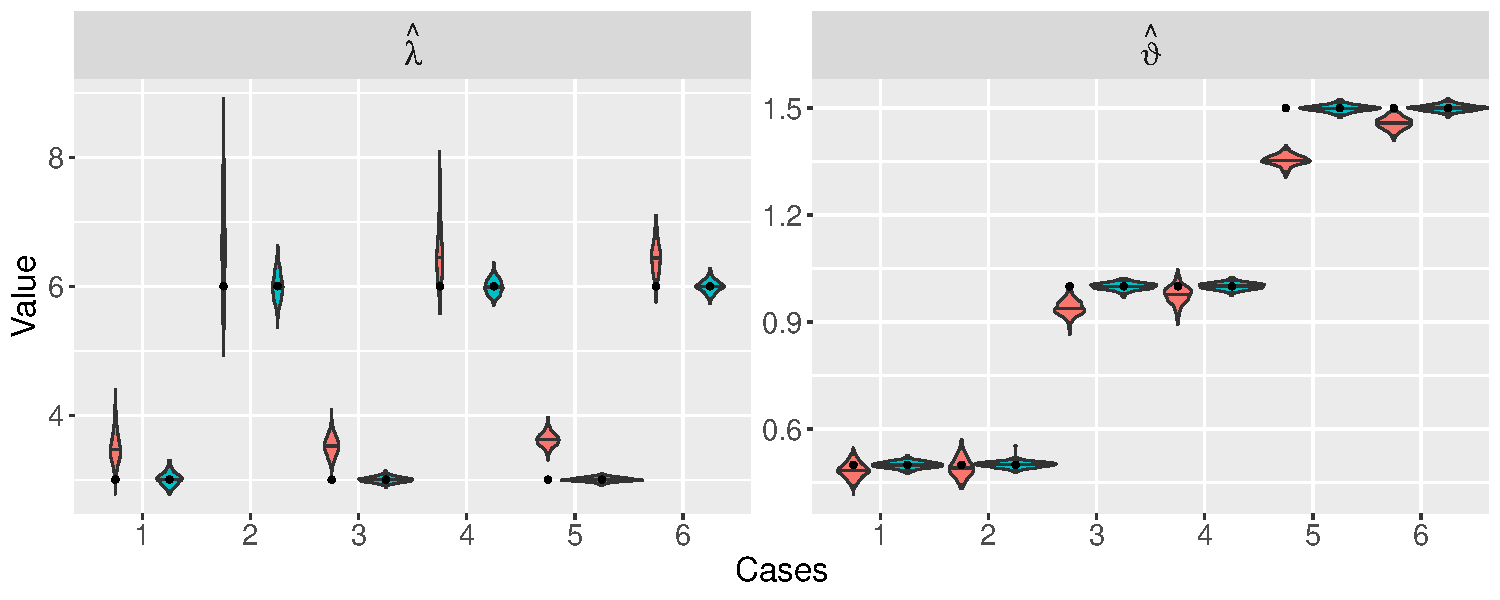
\includegraphics[width=1\textwidth]{simulation_est_boxplots_final_BR_30.pdf}    
    \caption{Violin plots for 300 replicate estimates of $\bm \theta = \left(\lambda, \vartheta\right)$ for the Brown-Resnick process with $\lambda=3,6$ and $\vartheta=0.5,1,1.5$ using the spectral (red) and pairwise (blue) likelihoods. Black dots indicate the true values.}
    \label{fig:simulation_boxplot_BR}
\end{figure}
%

%%%%%%%%%%%%%%%%%%%%%%%%%%%%%%%%%%%%%%%
%%%%%%%%%%%%%%%%%%%%%%%%%%%%%%%%%%%%%%%
\subsection{Comparing the spectral likelihood and score matching approach}
%%%%%%%%%%%%%%%%%%%%%%%%%%%%%%%%%%%%%%%
%%%%%%%%%%%%%%%%%%%%%%%%%%%%%%%%%%%%%%%

% \begin{figure}[ht]
%     \centering
%     \includegraphics[width=1\textwidth,page=5]{simulation_pareto_violin_logskew_5.pdf}
%     \includegraphics[width=1\textwidth,page=8]{simulation_pareto_violin_logskew_5.pdf}
%     \caption{Violin plots for the score matching (red) and spectral likelihood (blue) estimates of $\lambda$ (top) and  $b_2$ (bottom) for the skewed Brown-Resnick $r$-Pareto process with $L_3$ norm risk functional and the same parameter combinations as in Figure~4 of the main manuscript. Black dots indicate the parameter true values.}
% \end{figure}
%
% %
% \begin{figure}[ht]
%     \centering
%     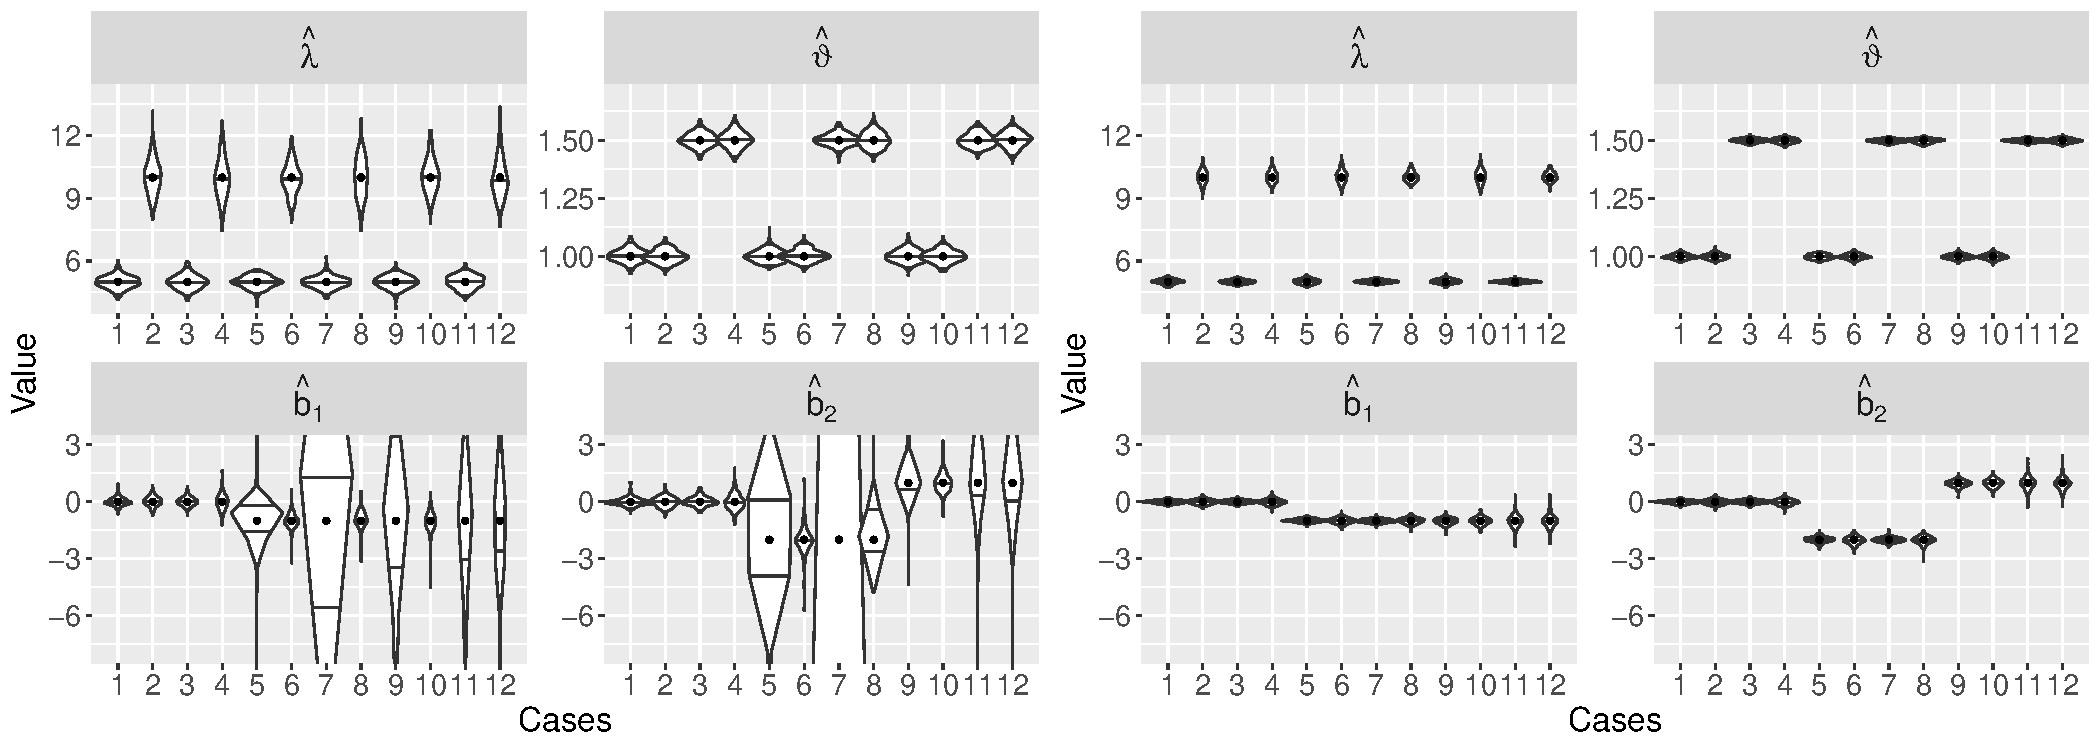
\includegraphics[width=1\textwidth,page=1]{simulation_pareto_violin__5_Inf_Inf.pdf}    
%     \caption{Violin plots for the score matching (left) and spectral likelihood (right) estimates of $\bm \theta= \left(\lambda, \vartheta,  b_1, b_2\right)$ for the skewed Brown-Resnick $r$-Pareto process with $L_1$ norm risk functional and the same parameter combinations as in Figure~4 of the main manuscript. Black dots indicate the parameter true values.}
%     \label{fig:simulation_boxplot_rpareto_skewedBR}
% \end{figure}
%
\begin{figure}[ht]
    \centering
    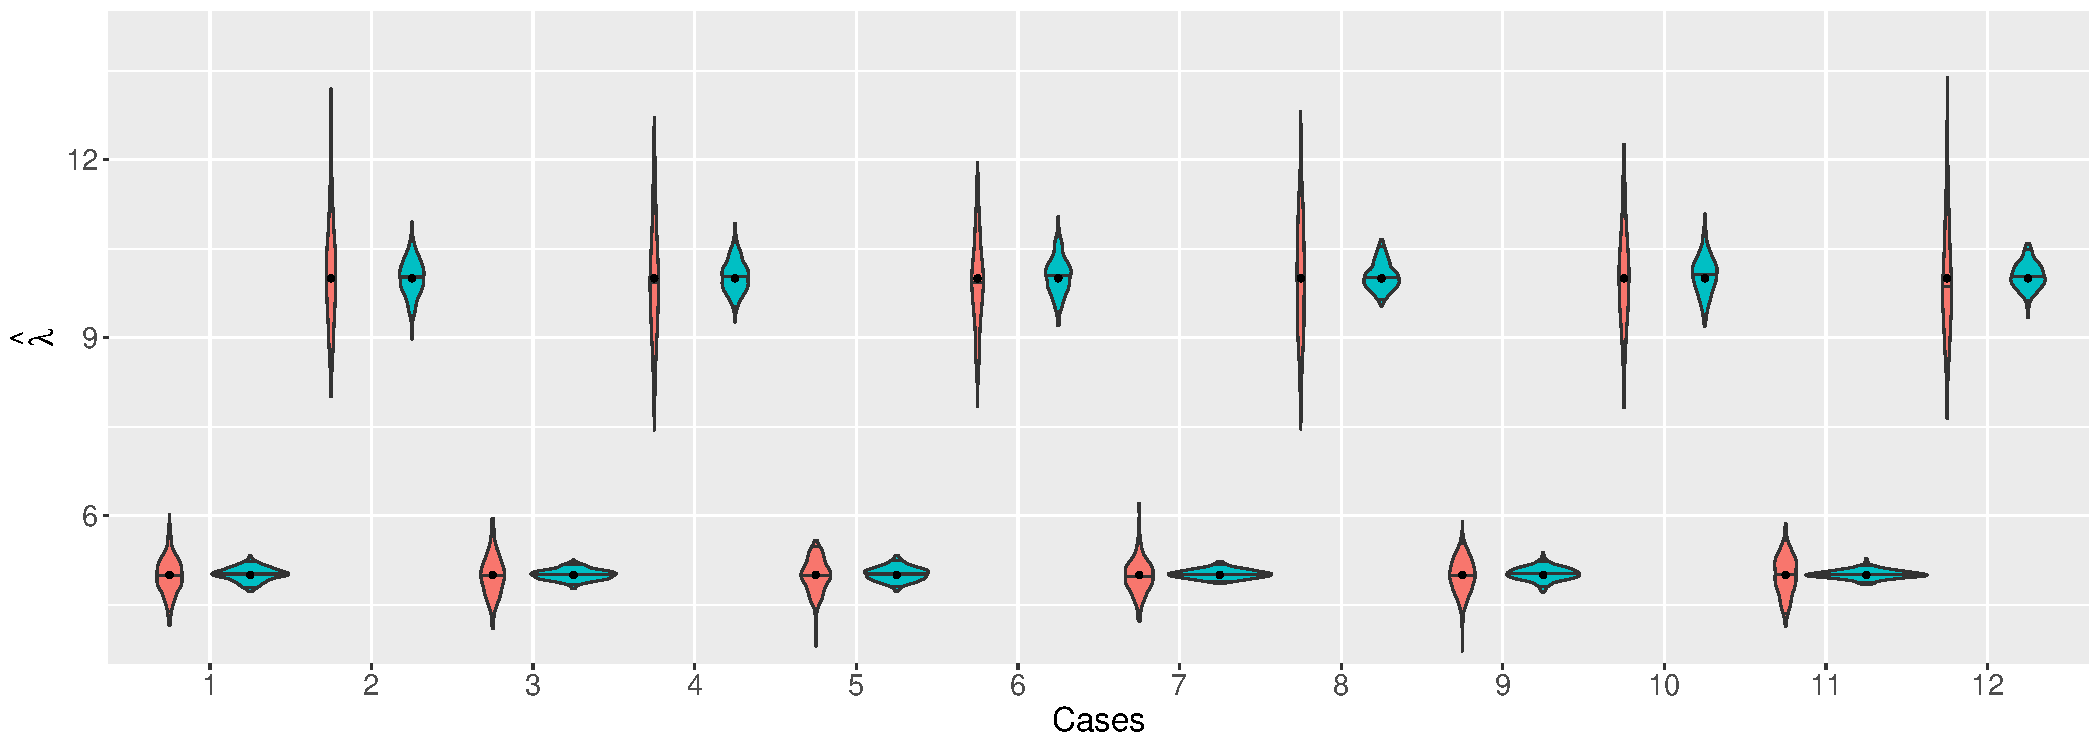
\includegraphics[width=0.9\textwidth,page=1]{simulation_pareto_violin_logskew_5.pdf}
    % \includegraphics[width=0.9\textwidth,page=2]{simulation_pareto_violin_logskew_5.pdf}
    % \includegraphics[width=0.9\textwidth,page=3]{simulation_pareto_violin_logskew_5.pdf}
    \includegraphics[width=0.9\textwidth,page=4]{simulation_pareto_violin_logskew_5.pdf}
    \caption{Violin plots for the score matching (red) and spectral likelihood (blue) estimates of $\bm \theta= \left(\lambda, b_2\right)$ (top to bottom) for the skewed Brown-Resnick $r$-Pareto process with $L_1$ norm risk functional and the same parameter combinations as in Figure~4 of the main manuscript. Black dots indicate the parameter true values.}
\end{figure}


%After considering the skewed Brown-Resnick $r$-Pareto process, 
We now generate $2,000$ samples from the truncated extremal-$t$ $r$-Pareto process on a $8\times8$ grid with $8$ parameter combinations using $\lambda=(3,5)$, $\vartheta=(1,1.5)$, and $\nu=2,3$ and $L_1$ norm as the risk functional. The model is fitted using both the score matching and spectral likelihood approaches with the outputs illustrated in Figure~\ref{fig:simulation_boxplot_rpareto_truncT} when the $L_1$-norm risk functional are used. 
%
We first note that there is barely any change in the performance of the estimators depending on the risk functional. Both estimation methods yield almost unbiased estimates for the smoothness parameter $\vartheta$. Some bias is however present for the estimation of the range parameter $\lambda$, with the spectral likelihood producing about $20\%$ relative bias, while the score matching method again shows numerical instability.
%
Again, the spectral likelihood shows greater computational efficiency ($126$ seconds on 3 CPU cores), being about $11$ times faster that the score matching method.

% \begin{figure}[!ht]
%     \centering
%     \includegraphics[width=1\textwidth,page=4]{simulation_pareto_violin__5_Inf_Inf.pdf}
%     \includegraphics[width=1\textwidth,page=3]{simulation_pareto_violin__5_Inf_Inf.pdf}
%     \caption{Violin plots for the score matching (left panels) and spectral likelihood (right panels) estimates of $\bm \theta= \left(\log(\lambda), \vartheta\right)$ for the truncated extremal-$t$ $r$-Pareto processes with $L_3$ norm (top) and $L_1$ norm (bottom) risk functional, where $\lambda=c(3,5),\vartheta=(1,1.5)$ and $\nu$ is fixed to be either 2 (case 1--4) or 3 (case 5--8). Black dots indicate the true values.}
%     \label{fig:simulation_boxplot_rpareto_truncT}
% \end{figure}
\begin{figure}[!ht]
    \centering
    % \includegraphics[width=0.9\textwidth,page=3]{simulation_pareto_violin_truncT_5.pdf}
    % \includegraphics[width=0.9\textwidth,page=4]{simulation_pareto_violin_truncT_5.pdf}
    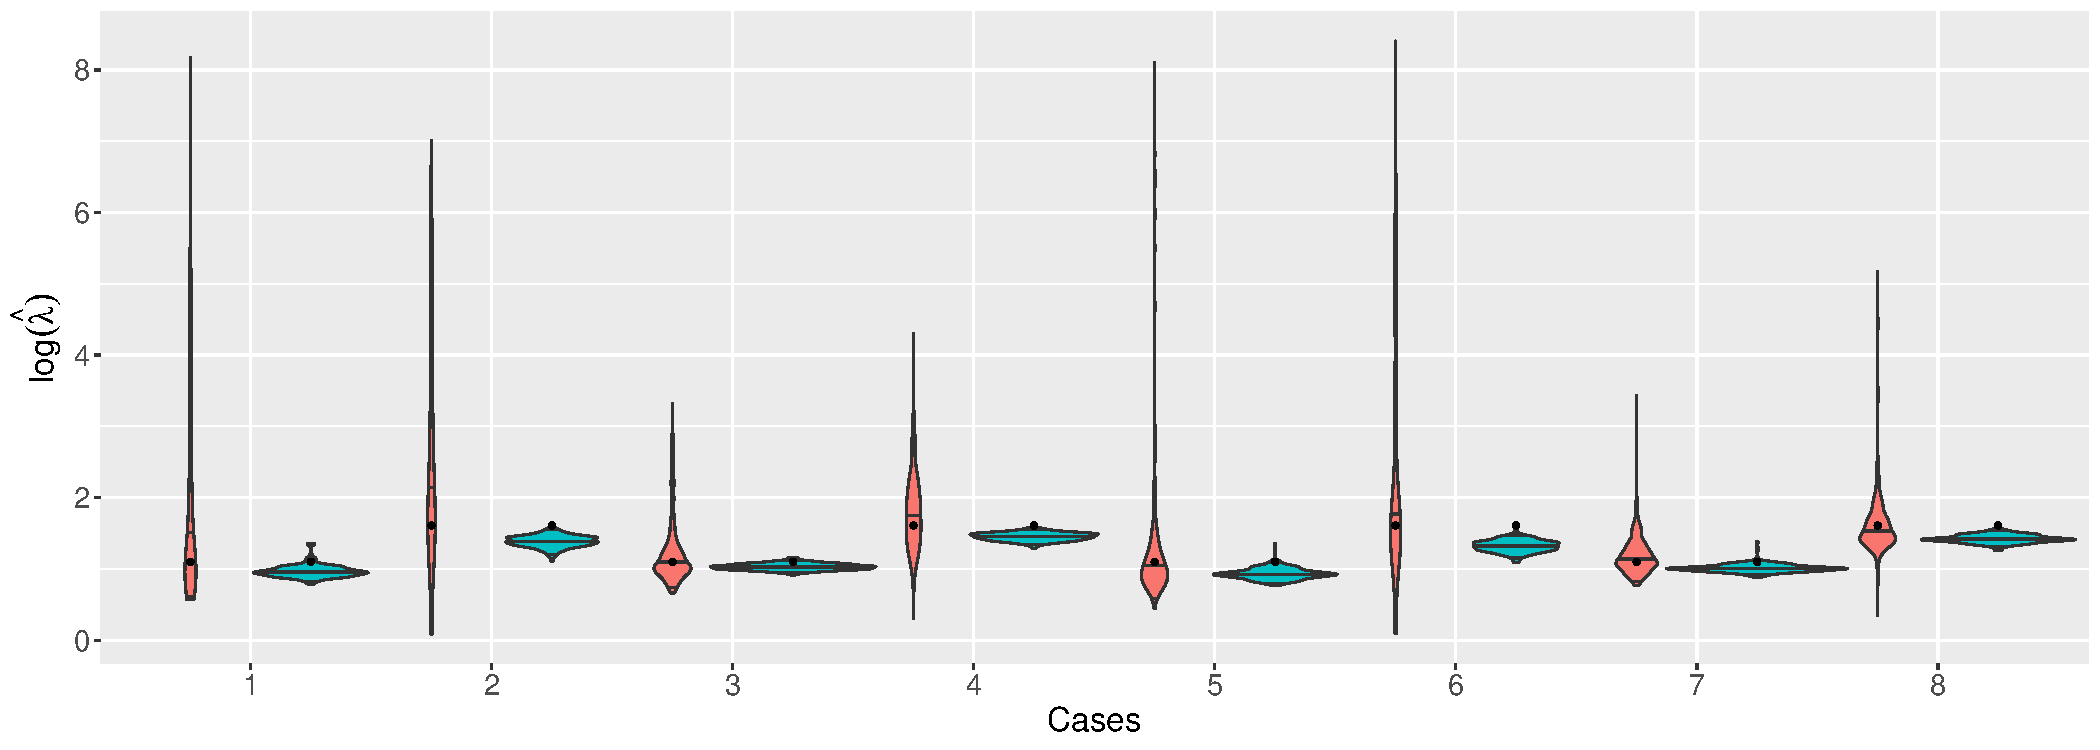
\includegraphics[width=0.9\textwidth,page=1]{simulation_pareto_violin_truncT_5.pdf}
    \includegraphics[width=0.9\textwidth,page=2]{simulation_pareto_violin_truncT_5.pdf}
    \caption{Violin plots for the score matching (red) and spectral likelihood (blue) estimates of $\bm \theta= \left(\log(\lambda), \vartheta\right)$ for the truncated extremal-$t$ $r$-Pareto processes with $L_1$ norm risk functional, where $\lambda=c(3,5),\vartheta=(1,1.5)$ and $\nu$ is fixed to be either 2 (case 1--4) or 3 (case 5--8). Black dots indicate the true values.}
    \label{fig:simulation_boxplot_rpareto_truncT}
\end{figure}

%%%%%%%%%%%%%%%%%%%%%%%%%%%%%%%%%%%%%%%
%%%%%%%%%%%%%%%%%%%%%%%%%%%%%%%%%%%%%%%
%%%%%%%%%%%%%%%%%%%%%%%%%%%%%%%%%%%%%%%
\section{Real-world applications}
%%%%%%%%%%%%%%%%%%%%%%%%%%%%%%%%%%%%%%%
%%%%%%%%%%%%%%%%%%%%%%%%%%%%%%%%%%%%%%%
%%%%%%%%%%%%%%%%%%%%%%%%%%%%%%%%%%%%%%%

See Figure \ref{fig:extcoef_application_florida2}.

\begin{figure}[!ht]
    \centering
    \begin{subfigure}{0.45\textwidth}
        \centering
        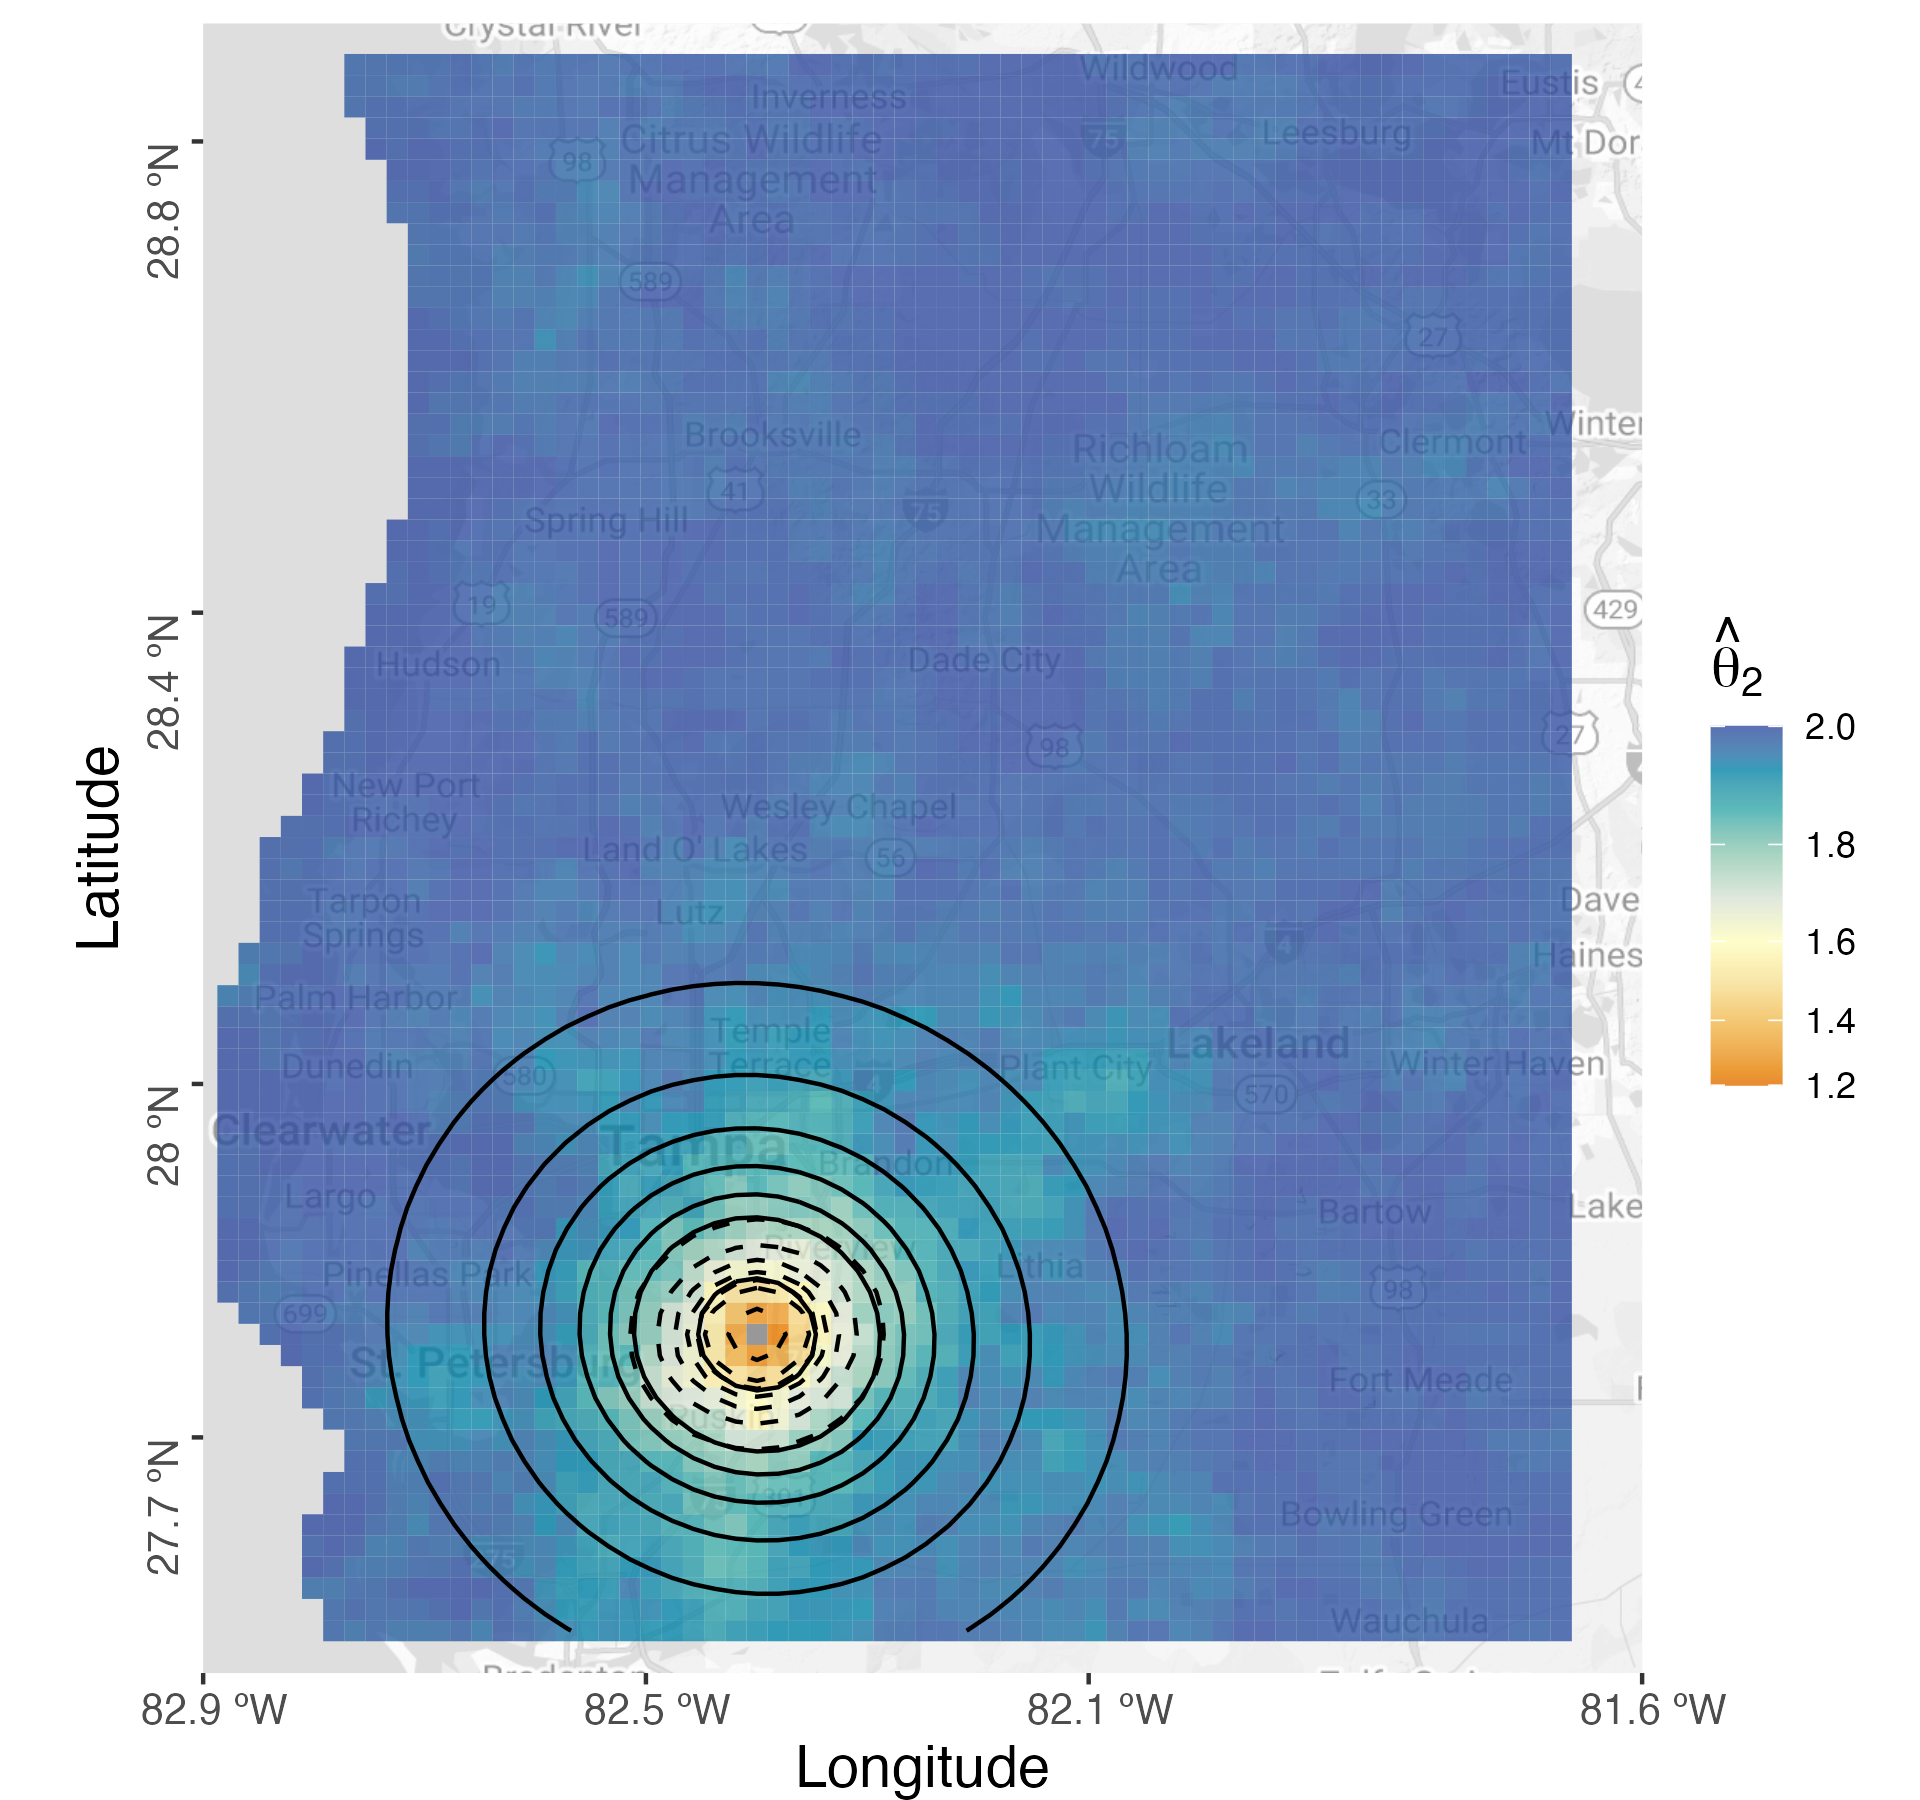
\includegraphics[width=1\textwidth]{florida/florida_extcoef2_3_008.png}
    \end{subfigure}%
    \begin{subfigure}{0.45\textwidth}
        \centering
        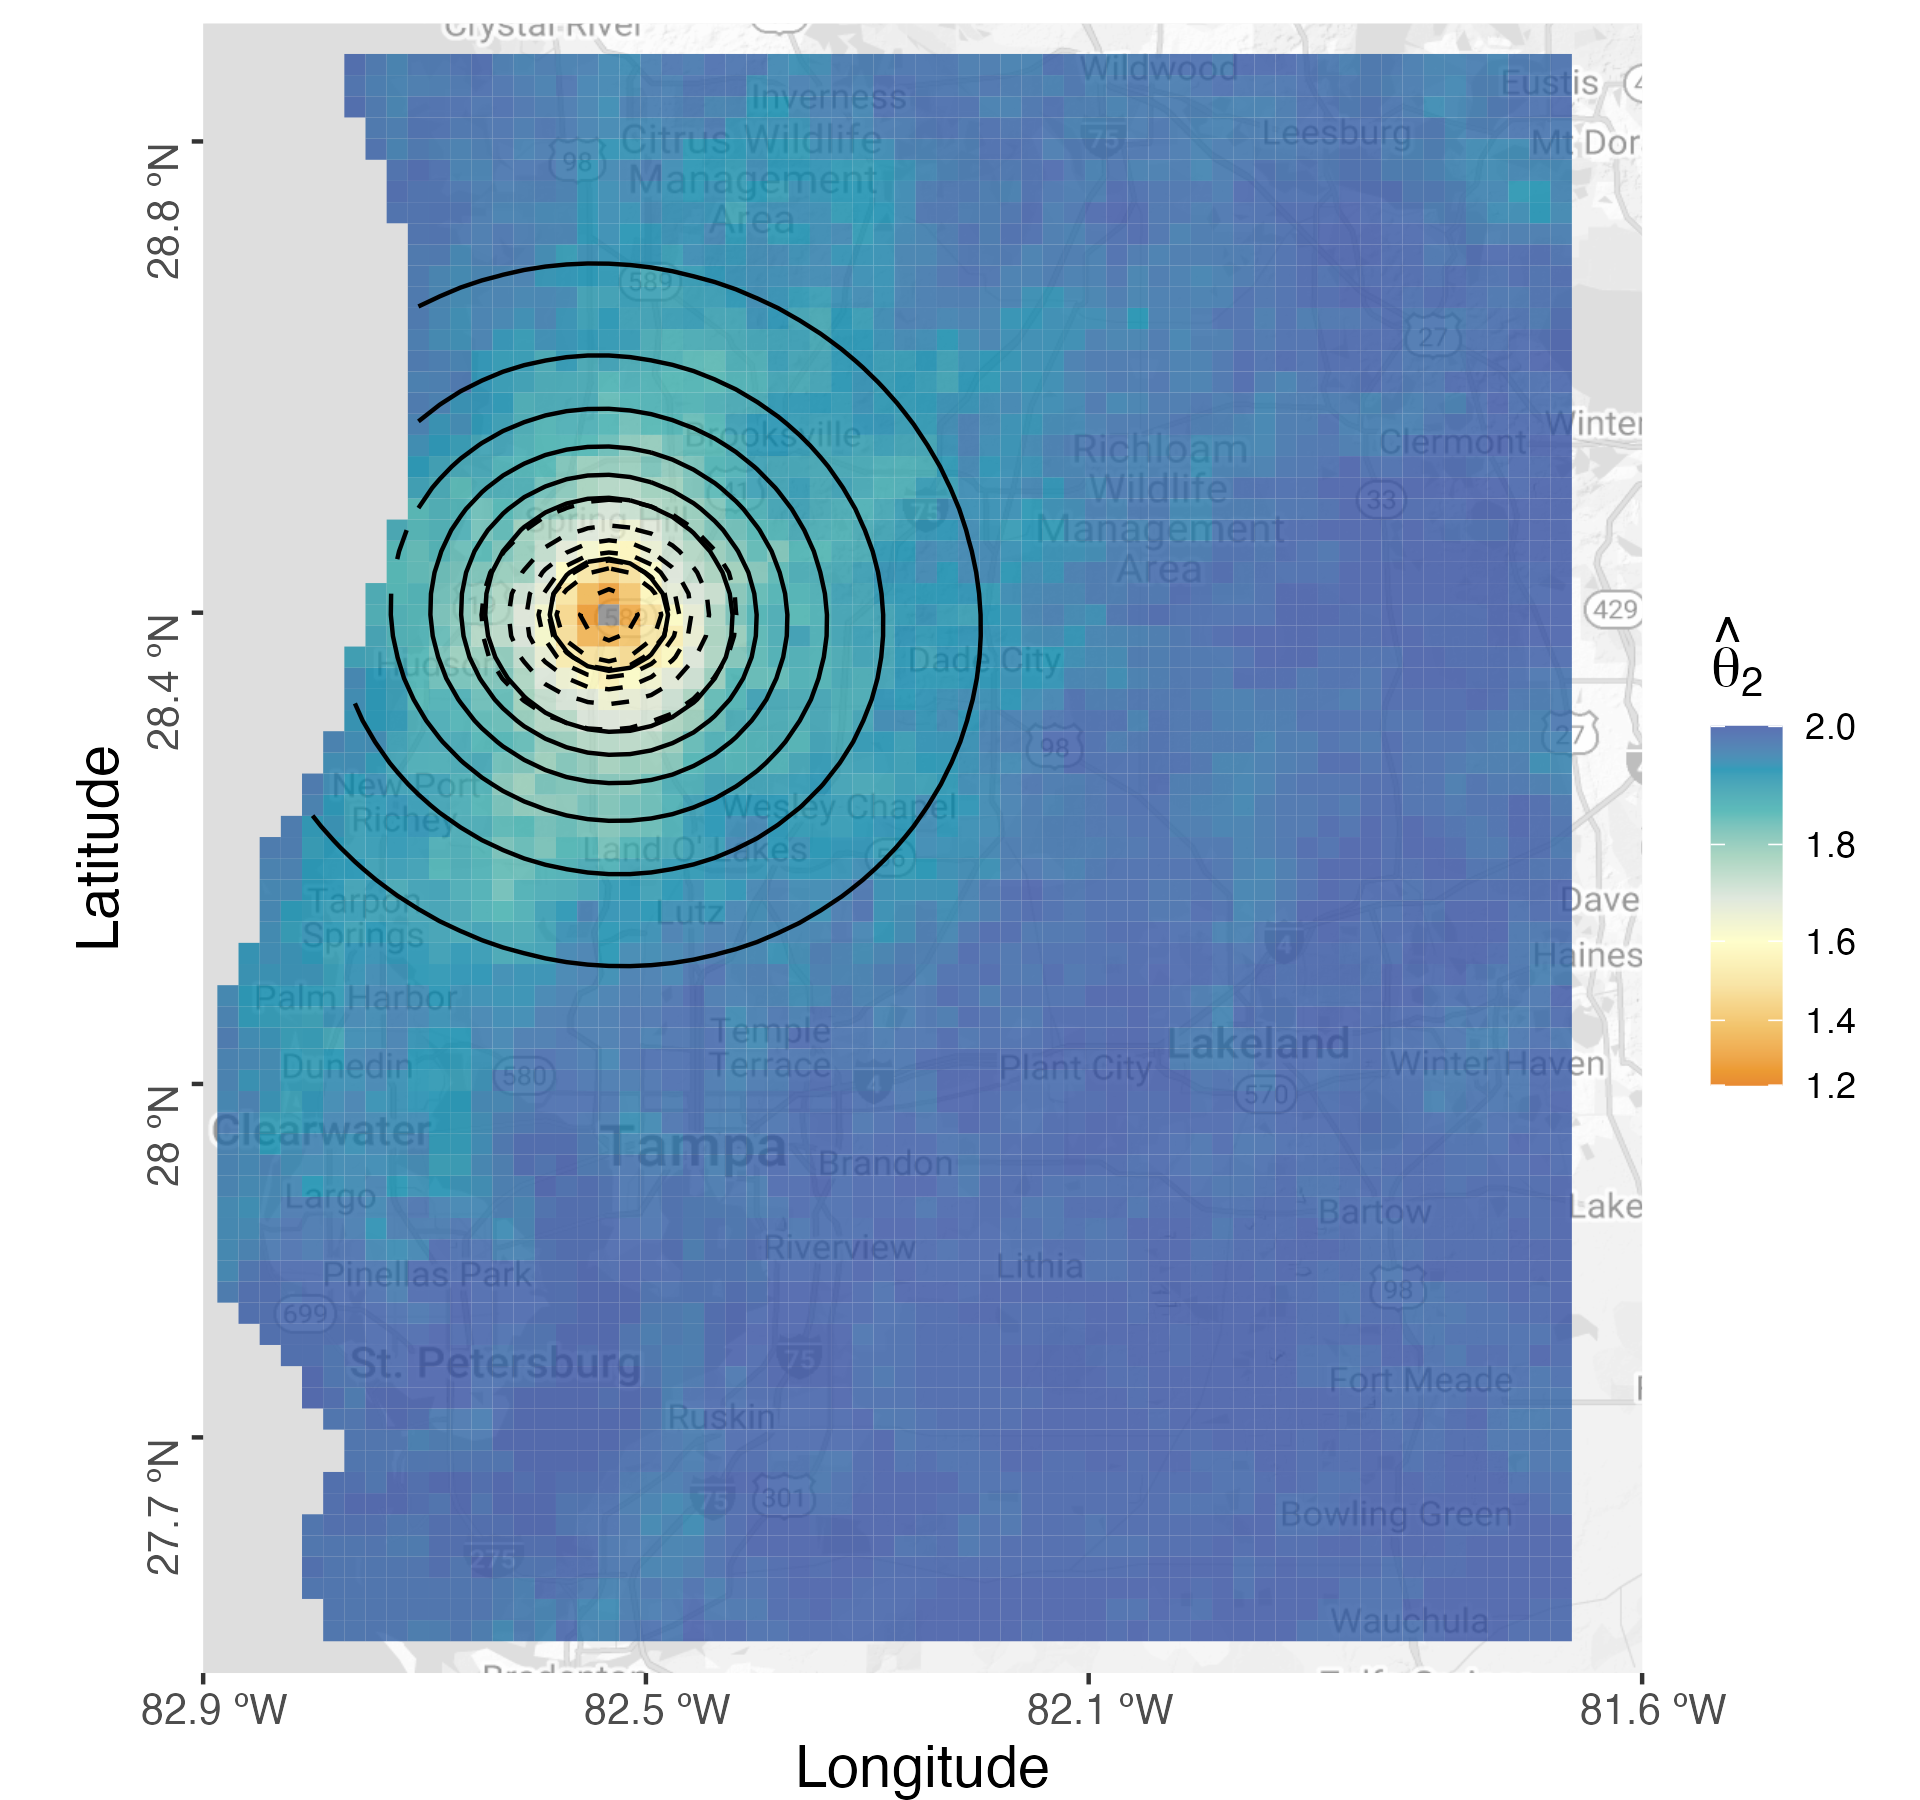
\includegraphics[width=1\textwidth]{florida/florida_extcoef2_3_038.png}
    \end{subfigure}
    % \begin{subfigure}{0.45\textwidth}
    %     \centering
    %     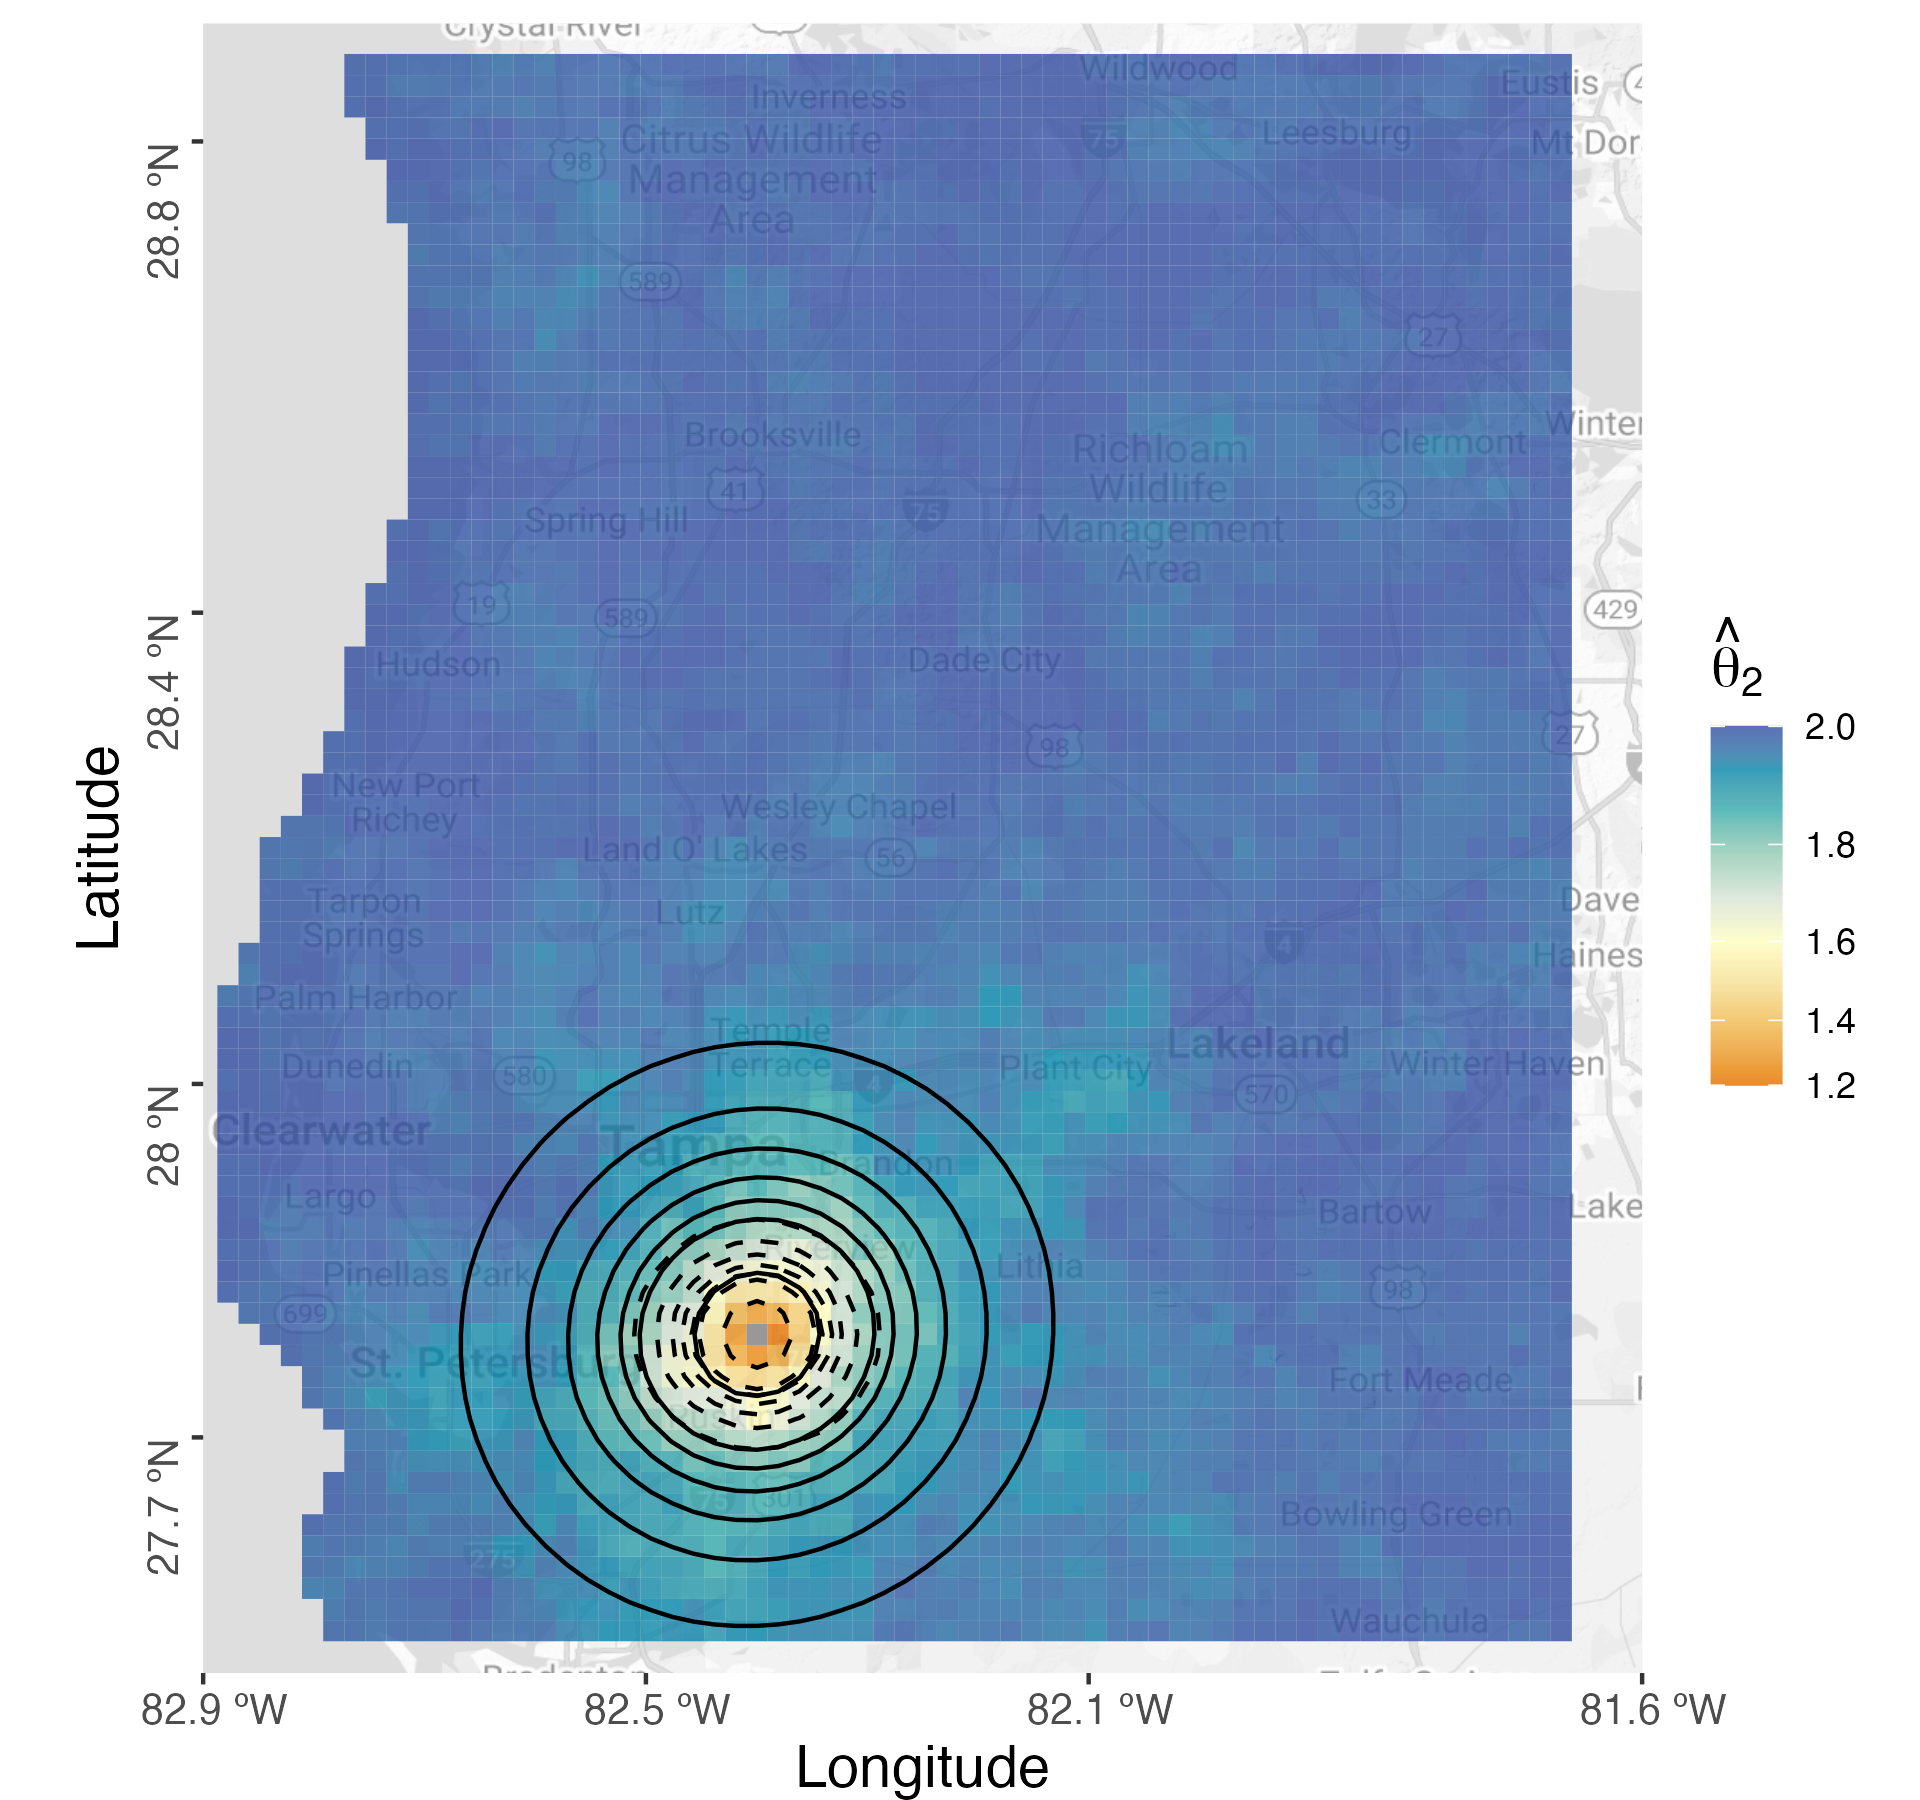
\includegraphics[width=1\textwidth]{florida/florida_extcoef2_4_008.png}
    % \end{subfigure}
    % \begin{subfigure}{0.45\textwidth}
    %     \centering
    %     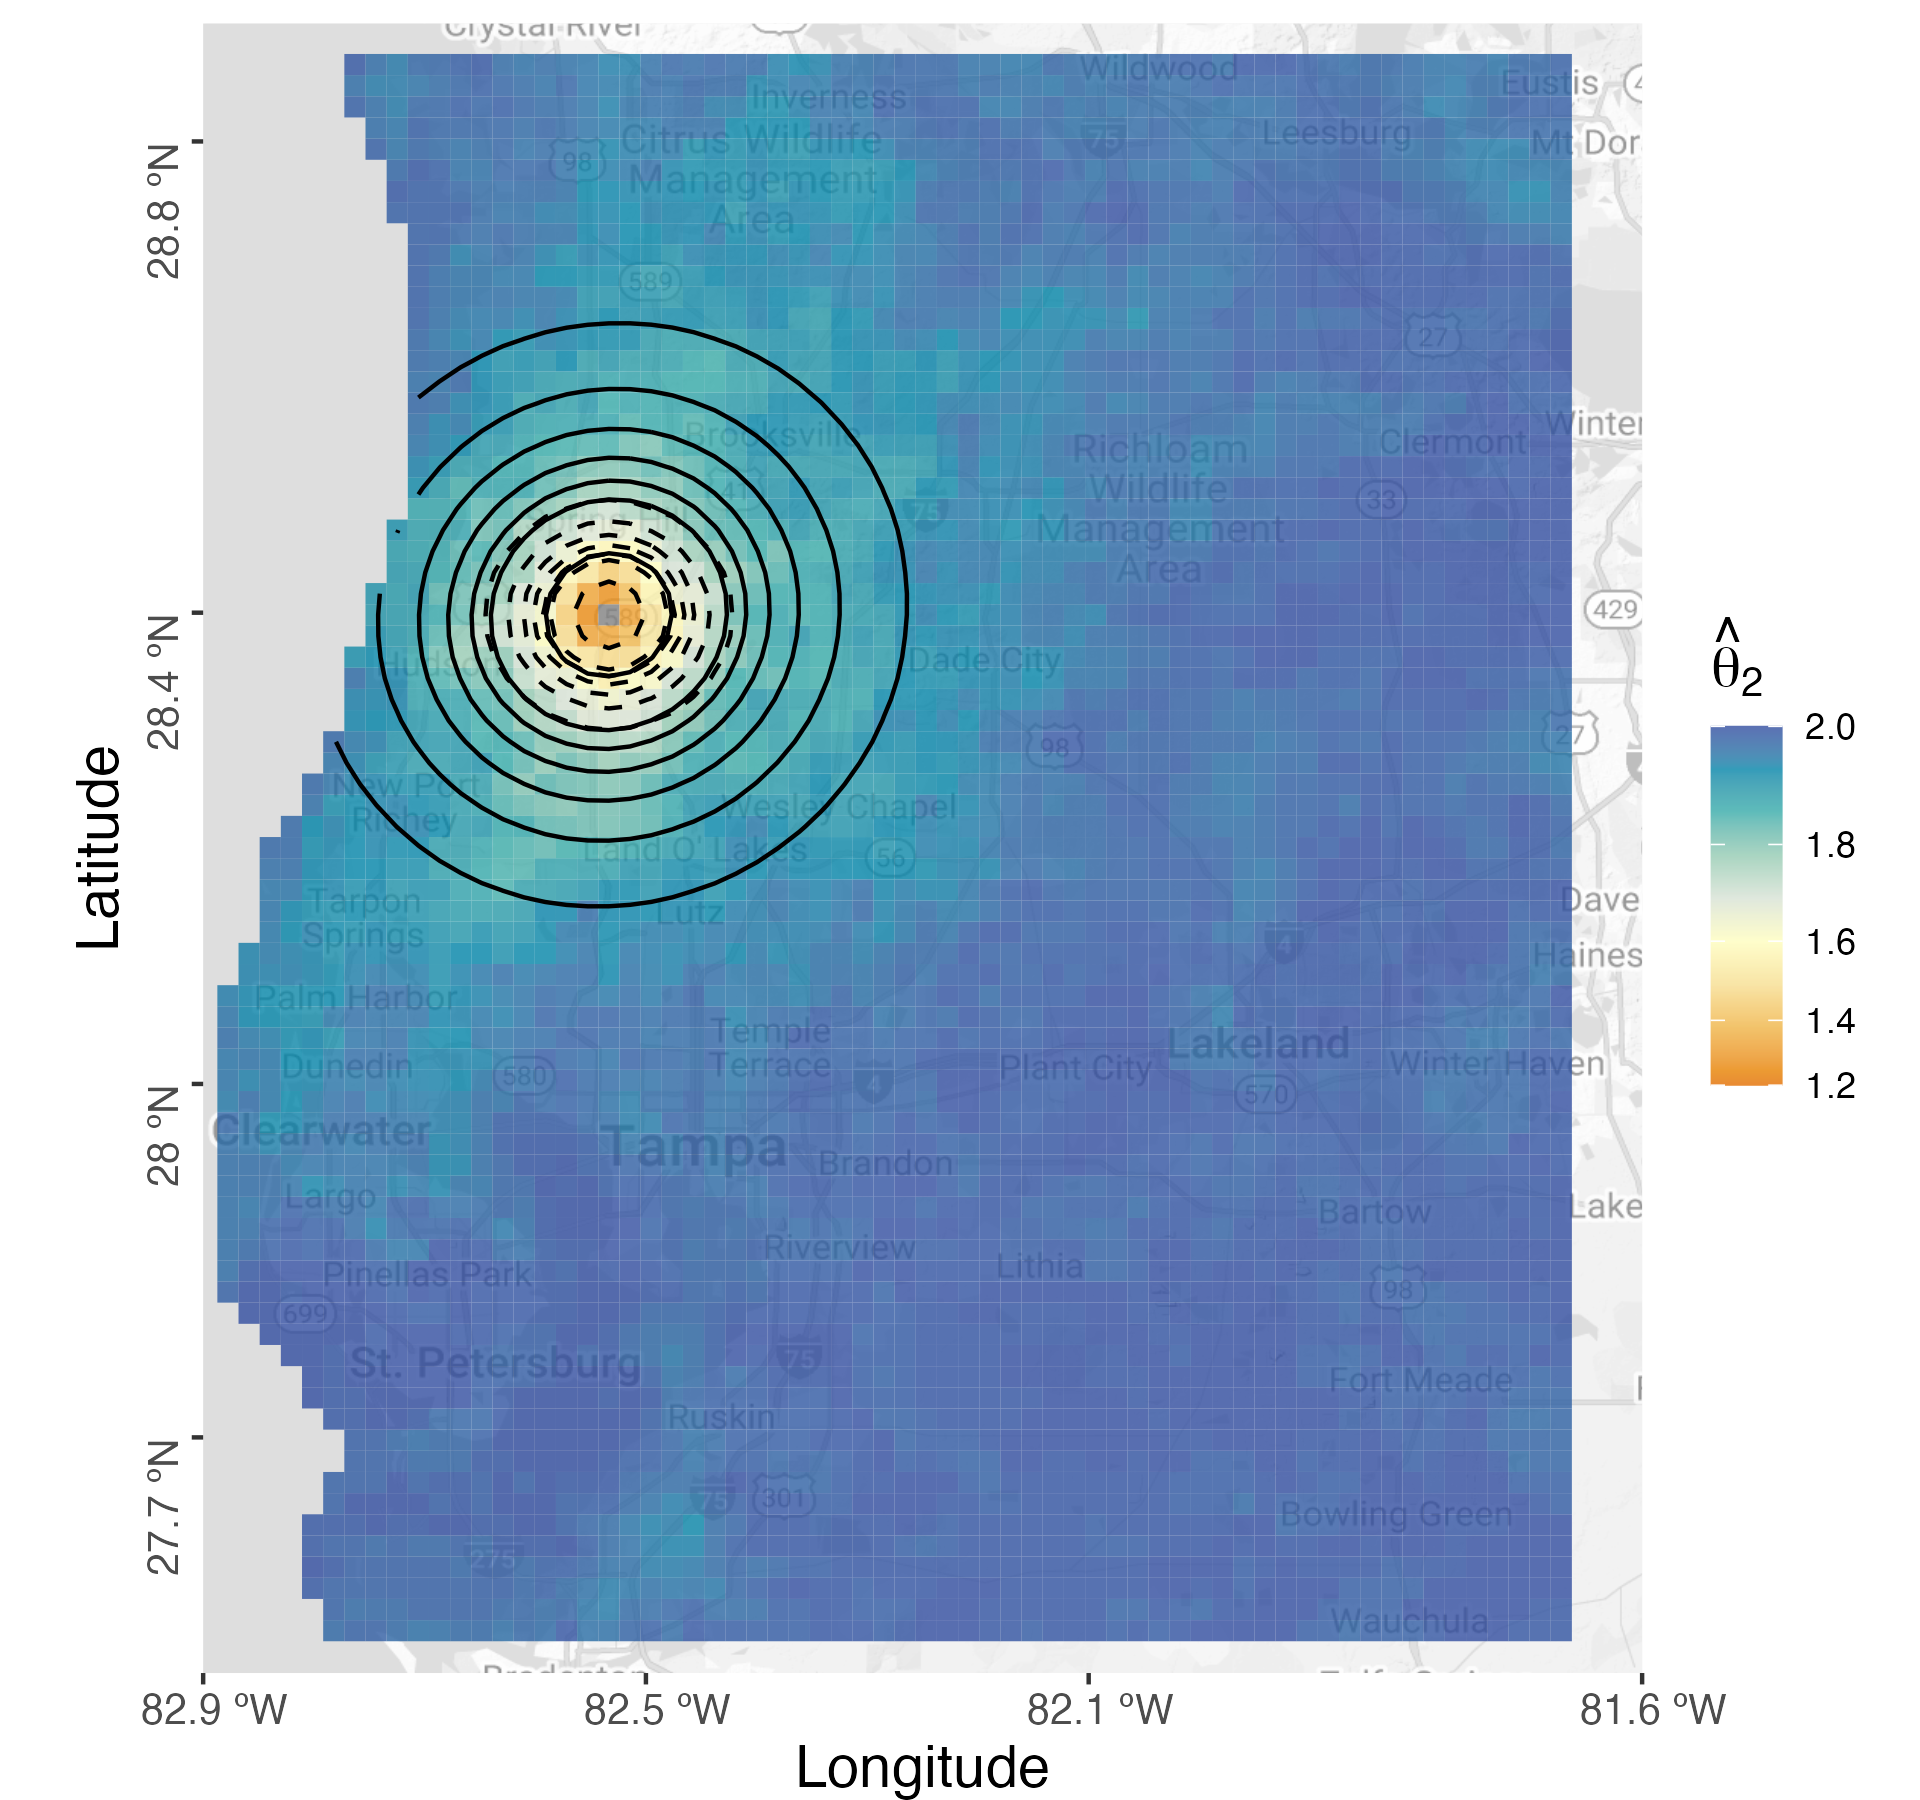
\includegraphics[width=1\textwidth]{florida/florida_extcoef2_4_038.png}
    % \end{subfigure}
    \caption{\small Maps of bivariate empirical extremal coefficients (shading) with respect to two different reference points (columns), and contours of the extremal coefficient of the Brown-Resnick $r$-Pareto model fitted using the spectral likelihood (solid line) and score matching approach (dashed line) on the Florida rainfall data.}
    \label{fig:extcoef_application_florida2}
\end{figure}

\begin{figure}[!ht]
    \centering
    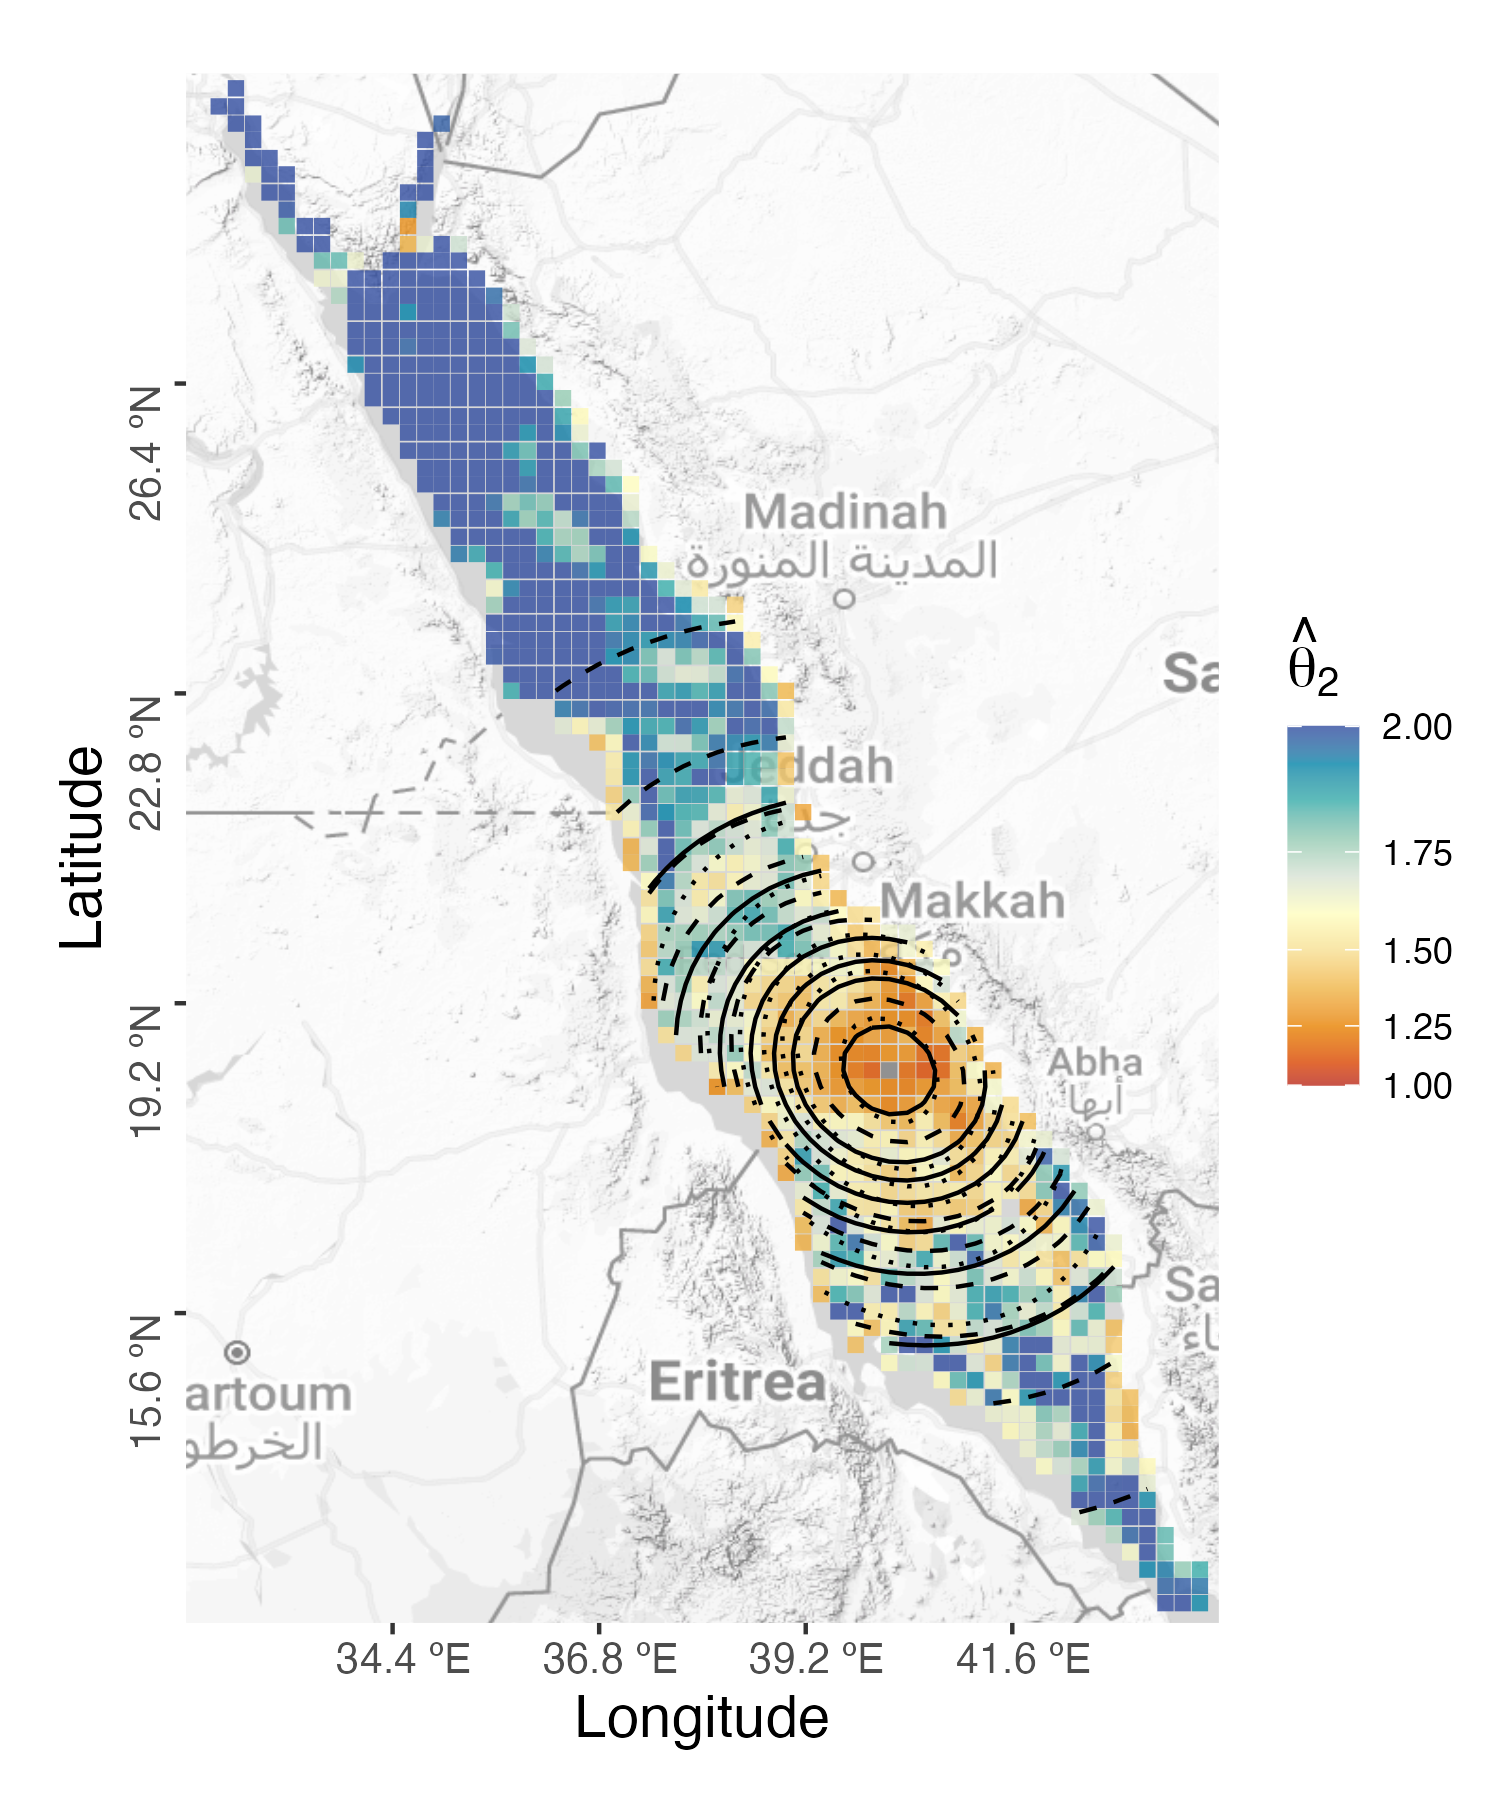
\includegraphics[width=0.49\textwidth]{RedSea2/RedSea_extcoef2_2_035.png}
    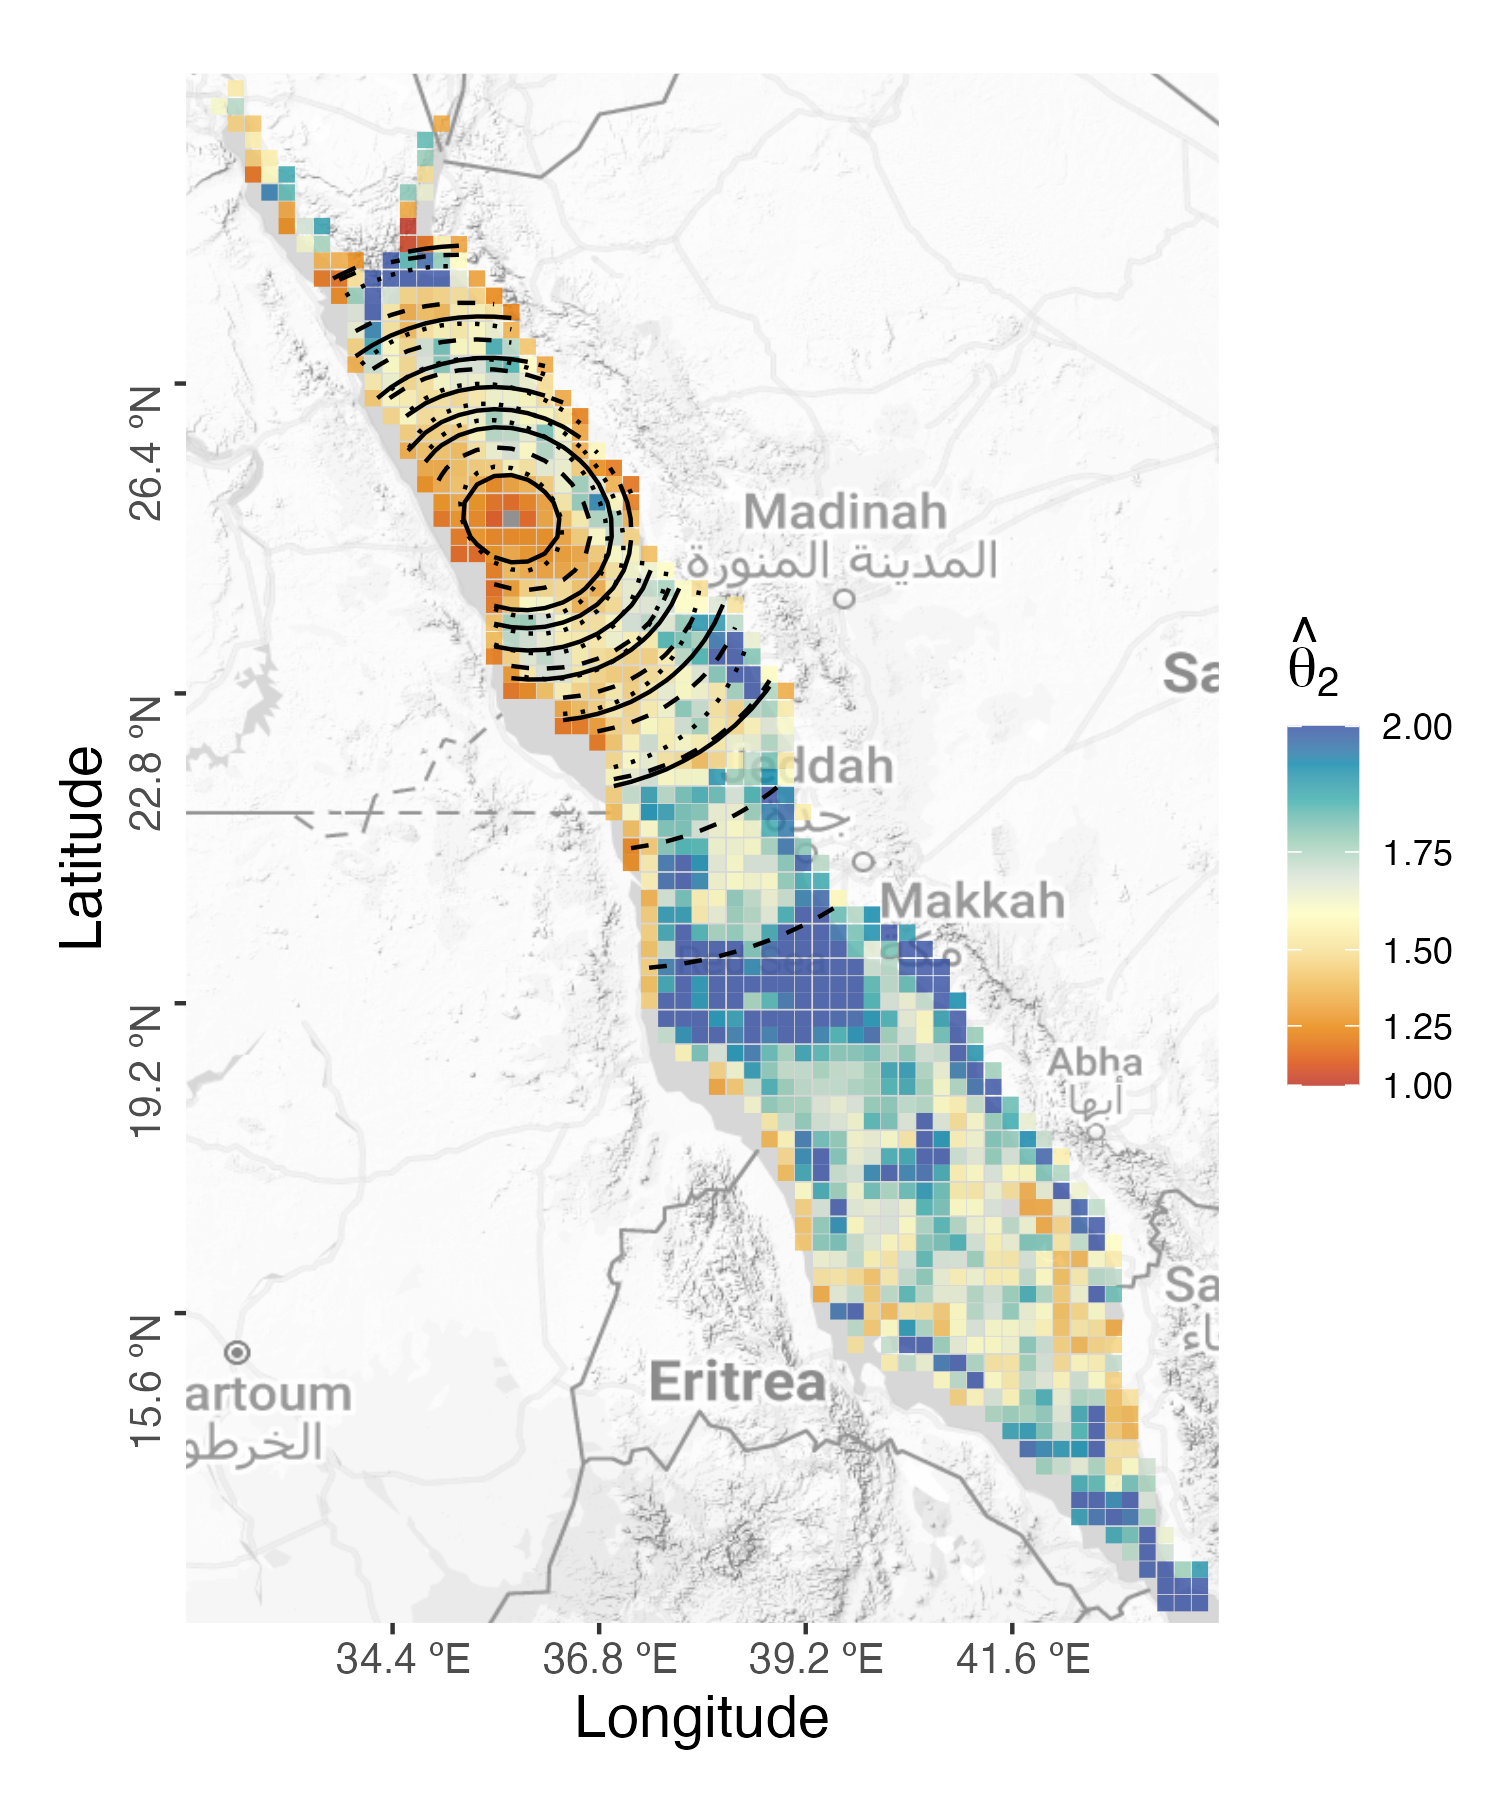
\includegraphics[width=0.49\textwidth]{RedSea2/RedSea_extcoef2_2_082.png}
    \caption{\small Maps of the bivariate empirical extremal coefficient (shading) with respect to two reference locations (left and right panels) with contours curves of the Brown-Resnick extremal coefficient fitted using the spectral likelihood (solid), pairwise composite likelihood (dotted) and Vecchia approximations (dashed).}
    \label{fig:extcoef_application_redsea_BR}
\end{figure}

\newpage

\bibliographystyle{CUP}
\bibliography{Total.bib}
\end{document}